\documentclass[12pt,a4paper]{article}
\usepackage[utf8]{inputenc}
\usepackage{amsmath}
\usepackage{amsfonts}
\usepackage{amssymb}
\usepackage{graphicx}
\usepackage{cite}
\usepackage[hidelinks]{hyperref}
\usepackage{geometry}
\usepackage{booktabs}
\usepackage{tocloft}
\usepackage{fancyhdr}
\usepackage{titlesec}
\usepackage{xcolor}
\usepackage{setspace}
\usepackage{esvect}
\usepackage{tikz}
\usetikzlibrary{shapes,arrows,positioning,fit,calc}

\geometry{
 a4paper,
 left=20mm,
 right=20mm,
 top=25mm,
 bottom=25mm,
 headheight=14pt,
}

% Custom colors
\definecolor{titlecolor}{RGB}{0,51,102}
\definecolor{sectioncolor}{RGB}{0,102,153}

% Section formatting
\titleformat{\section}
  {\Large\bfseries\color{sectioncolor}}
  {\thesection}{1em}{}[\titlerule]

\titleformat{\subsection}
  {\large\bfseries\color{sectioncolor}}
  {\thesubsection}{1em}{}

\titleformat{\subsubsection}
  {\normalsize\bfseries\color{sectioncolor}}
  {\thesubsubsection}{1em}{}

% Header and footer
\pagestyle{fancy}
\fancyhf{}
\fancyhead[L]{\small\textit{Stock Price Prediction using Algorithmic Trading}}
\fancyhead[R]{\small\thepage}
\fancyfoot[C]{\small Department of Computer Science, Sister Nivedita University}
\renewcommand{\headrulewidth}{0.4pt}
\renewcommand{\footrulewidth}{0.4pt}

% Table of contents formatting
\renewcommand{\cftsecfont}{\bfseries}
\renewcommand{\cftsecpagefont}{\bfseries}
\setlength{\cftbeforesecskip}{8pt}

% Line spacing
\setstretch{1.15}

\begin{document}

% Custom title page
\begin{titlepage}
    \centering
    \vspace*{1cm}
    
    % University logo placeholder
    \begin{figure}[h]
        \centering
        
\includegraphics[width=0.35\textwidth]{pdfs/extract_text copy.png}
    \end{figure}
    
    \vspace{1cm}
    
    % Title Section with rules
    \rule{\linewidth}{0.5mm} \\[0.4cm]
    {\huge \bfseries \color{titlecolor} Stock Price Prediction using Algorithmic Trading} \\[0.2cm]
    {\Large \color{sectioncolor} A Comprehensive Literature Review} \\[0.4cm]
    \rule{\linewidth}{0.5mm}
    
    \vspace{2cm}
    
    % Author Section
    {\Large \textit{Submitted by}} \\[0.5cm]
    {\large \bfseries
    \begin{tabular}{c}
        Anik Das \\
        Agnirudra Banerjee \\
        Mohar Mukherjee \\
        Bibhas Roy
    \end{tabular}
    }
    
    \vfill
    
    % Degree and Dept Info
    {\large Submitted in partial fulfillment of the requirements for the degree of} \\[0.5cm]
    {\Large \textsc{Bachelor of Technology}} \\[0.2cm]
    {\large in} \\[0.2cm]
    {\Large \textsc{Computer Science and Engineering}}
    
    \vspace{1.5cm}
    
    % Institution
    {\Large \bfseries \color{titlecolor} Sister Nivedita University} \\[0.2cm]
    {\large Newtown, Kolkata, West Bengal}
    
    \vspace{1cm}
    
    {\large \textbf{2025}}
    
\end{titlepage}

% Second Title Page / Submission Page
\begin{titlepage}
    \centering
    \vspace*{0.5cm}
    
    % University logo
    \begin{figure}[h]
        \centering
        
\includegraphics[width=0.35\textwidth]{pdfs/extract_text copy.png}
    \end{figure}
    
    \vspace{0.5cm}
    
    {\huge \bfseries \color{titlecolor} Stock Price Prediction using Algorithmic Trading} \\[0.5cm]
    
    {\large Project Submitted in Partial Fulfillment of the Requirements for the Degree of} \\[0.3cm]
    {\Large \textsc{Bachelor of Technology (CSE)}}
    
    \vspace{1.5cm}
    
    \renewcommand{\arraystretch}{1.8}
    \begin{table}[h]
        \centering
        \begin{tabular}{l l l}
            \textbf{Name} & \textbf{Enrollment} & \textbf{Email ID} \\
            Agnirudra Banerjee & 2211200010029 & agnirudrabanerjee777@gmail.com \\
            Bibhas Roy & 2211200010001 & abc.3gbibhas@gmail.com \\
            Mohar Mukherjee & 2211200010010 & MOHARMUKHERJEE2004@gmail.com \\
            Anik Das & 2211200010038 & anik200365@gmail.com \\
        \end{tabular}
    \end{table}
    
    \vspace{0.5cm}
    
    {\textbf{Submission Date:} 21-November, 2025}
    
    \vspace{1cm}
    
    {\textit{Under the supervision of}} \\[0.2cm]
    {\textbf{Dr. Soma Datta}} \\[0.1cm]
    {Assistant Professor} \\[0.1cm]
    {Department of Computer Science} \\[0.1cm]
    {Sister Nivedita University, Newtown} \\[0.1cm]
    {Kolkata, West Bengal}
    
    \vfill
    
    % Institution Footer
    {\Large \bfseries \color{titlecolor} Sister Nivedita University} \\[0.2cm]
    {\large Newtown, Kolkata, West Bengal}
    
    \vspace{0.5cm}
    
    {\large \textbf{November, 2025}}
\end{titlepage}

% Reset page numbering
\pagenumbering{roman}
\setcounter{page}{1}

% Declaration Page
\newpage
\begin{center}
    \vspace*{1cm}
    {\Large \bfseries \color{titlecolor} DECLARATION}
    \vspace{1cm}
\end{center}

\noindent We hereby declare that the project work entitled \textbf{``Stock Price Prediction using Algorithmic Trading''} submitted to the Department of Computer Science, Sister Nivedita University, is a record of an original work done by us under the supervision of \textbf{Dr. Soma Datta}, Assistant Professor, Department of Computer Science, Sister Nivedita University.

\vspace{0.5cm}
\noindent This project work is submitted in partial fulfillment of the requirements for the award of the degree of \textbf{Bachelor of Technology in Computer Science and Engineering}. The results embodied in this report have not been submitted to any other University or Institute for the award of any degree or diploma.

\vspace{2cm}

\begin{table}[h]
    \centering
    \begin{tabular}{p{6cm} p{6cm}}
        ...................................................... & ...................................................... \\
        \textbf{Agnirudra Banerjee} & \textbf{Bibhas Roy} \\[1cm]
        
        ...................................................... & ...................................................... \\
        \textbf{Mohar Mukherjee} & \textbf{Anik Das} \\
    \end{tabular}
\end{table}

\vspace{1cm}
\noindent \textbf{Place:} Kolkata \\
\noindent \textbf{Date:} November, 2025

% Certificate Page
\newpage
\begin{center}
    \vspace*{1cm}
    {\Large \bfseries \color{titlecolor} CERTIFICATE}
    \vspace{1cm}
\end{center}

\noindent This is to certify that the project report entitled \textbf{``Stock Price Prediction using Algorithmic Trading''} submitted by:

\vspace{0.5cm}
\begin{center}
    \begin{tabular}{l l}
        \textbf{Agnirudra Banerjee} & (ID: 2211200010029) \\
        \textbf{Bibhas Roy} & (ID: 2211200010001) \\
        \textbf{Mohar Mukherjee} & (ID: 2211200010010) \\
        \textbf{Anik Das} & (ID: 2211200010038) \\
    \end{tabular}
\end{center}
\vspace{0.5cm}

\noindent in partial fulfillment of the requirements for the award of the degree of \textbf{Bachelor of Technology in Computer Science and Engineering} of Sister Nivedita University, is a bona fide record of the work carried out under my supervision and guidance.

\vspace{3cm}

\noindent \rule{6cm}{0.4pt} \\
\noindent \textbf{Dr. Soma Datta} \\
Assistant Professor \\
Department of Computer Science \\
Sister Nivedita University, Newtown, Kolkata

\newpage

% Table of Contents
\tableofcontents
\newpage

% List of Figures
\listoffigures
\newpage

% List of Tables
\listoftables
\newpage

% Acknowledgement Page
\begin{center}
    \vspace*{1cm}
    {\Large \bfseries \color{titlecolor} ACKNOWLEDGEMENT}
    \vspace{1cm}
\end{center}

\noindent We would like to express our deep sense of gratitude and profound respect to our supervisor, \textbf{Dr. Soma Datta}, Assistant Professor, Department of Computer Science, Sister Nivedita University, for her valuable guidance, constant encouragement, and constructive criticism throughout the course of this project work. Her expertise and insight have been invaluable in shaping our understanding of the subject.

\vspace{0.5cm}
\noindent We are also grateful to the \textbf{Department of Computer Science} and \textbf{Sister Nivedita University} for providing us with the necessary facilities and an environment conducive to learning and research.

\vspace{0.5cm}
\noindent Finally, we would like to thank our families and friends for their unwavering support and encouragement during this endeavor.

\vspace{2cm}
\vspace{2cm}
\begin{table}[h]
    \centering
    \begin{tabular}{p{6cm} p{6cm}}
        ...................................................... & ...................................................... \\
        \textbf{Agnirudra Banerjee} & \textbf{Bibhas Roy} \\[1cm]
        
        ...................................................... & ...................................................... \\
        \textbf{Mohar Mukherjee} & \textbf{Anik Das} \\
    \end{tabular}
\end{table}

\newpage

% Abstract Page
\begin{center}
    \vspace*{1cm}
    {\Large \bfseries \color{titlecolor} ABSTRACT}
    \vspace{1cm}
\end{center}

\noindent The prediction of stock market prices is a challenging task due to the non-linear, volatile, and sentiment-driven nature of financial time series data. Traditional statistical models like ARIMA have limitations in capturing non-linear patterns, while deep learning models like LSTM excel at sequential data but may struggle with noise. Price-only models, regardless of architectural sophistication, are structurally blind to exogenous information shocks---such as earnings surprises, macroeconomic announcements, and shifts in public sentiment---until those shocks are already reflected in historical prices. This literature review comprehensively explores the evolution of stock prediction methodologies, with a specific focus on \textbf{Hybrid Models} that combine the strengths of multiple approaches (e.g., ARIMA-LSTM, CNN-LSTM), and extends the analysis to \textbf{Sentiment-Aware Hybrid Architectures} that integrate financial news sentiment into the prediction pipeline.

\vspace{0.5cm}
\noindent We analyze various hybrid architectures, comparing their mechanisms, strengths, and limitations. The review highlights how hybrid models consistently outperform standalone models by effectively handling both linear and non-linear components, as well as incorporating diverse data sources such as technical indicators and macroeconomic variables. Building on this foundation, we propose a sentiment-augmented extension of the SARIMA-XGBoost hybrid model that integrates a domain-adapted sentiment analysis pipeline featuring dual-head sarcasm correction, principled temporal alignment of news publication timestamps to trading days, and confidence-weighted sentiment aggregation. The system addresses critical gaps identified in modern sentiment analysis literature---including sarcasm and irony detection, tokenization drift in financial language, domain sensitivity, and uncertainty quantification---and feeds structured sentiment features into the XGBoost residual learning stage, enabling the model to capture linear trends, non-linear residual patterns, and sentiment-driven price dynamics within a unified three-component decomposition $y_t = L_t + N_t + E_t + \epsilon_t$. Furthermore, this document identifies research gaps in current methodologies, particularly regarding multimodal data integration, the lack of adaptive learning mechanisms for regime shifts, and the absence of robust risk-aware prediction frameworks. These identified gaps and the proposed sentiment-aware architecture lay the foundation for more robust and accurate stock prediction systems.

\newpage

% Main content starts here
\newpage
\pagenumbering{arabic}
\setcounter{page}{1}

\section{Introduction}

\subsection{Context of the Study}
The stock market is a part of the financial system. The stock market shows how the economy is doing and moves money to where it's needed. I find that predicting the stock market is hard. The stock market moves in complex ways, has swings, and does not follow a straight line. The stock market data is a time series that can change quickly. The stock prices move fast because they stock prices are affected by things. The stock prices react to how a company performs, to numbers to world events, to market mood and to investor behavior.

Traditional statistical models have been used for decades to forecast stock prices. Traditional statistical models often have trouble with market shifts, regime changes and non‑linear patterns in the data. The rise of machine learning and deep learning gives researchers tools to study the patterns. Machine learning and deep learning can handle patterns that traditional statistical models miss. I have seen that modern computational techniques can learn from large amounts of data. Modern computational techniques can find relationships that're hard to see with analysis or with classical statistical methods. When modern computational techniques look at years of data modern computational techniques can spot connections that no one would notice by just looking at the numbers or by using traditional statistical models.

However, even the most sophisticated price-based models---whether statistical, machine learning, or deep learning---share a fundamental structural limitation: they operate entirely on historical OHLCV (Open, High, Low, Close, Volume) features and derived technical indicators. These models have no mechanism to respond to sudden exogenous information shocks, such as a negative earnings surprise, a CEO resignation, or a macroeconomic policy change, until those shocks are already reflected in the price history. Financial markets are fundamentally information-processing systems where news, earnings announcements, analyst opinions, and public sentiment all contribute to price discovery. A model that can extract and quantify the sentiment embedded in financial news, and integrate it into its prediction pipeline, effectively gains advance information that price-only models lack.

Integrating sentiment analysis into financial prediction is not straightforward. Modern sentiment models suffer from several well-documented gaps: financial language contains domain-specific jargon, hedged expressions, and sarcasm that general-purpose sentiment models misinterpret; news publication timestamps do not directly align with trading day boundaries, creating temporal mismatch problems; most sentiment pipelines produce deterministic point estimates with no uncertainty quantification; and models trained on general corpora experience tokenization drift when applied to financial text. This work is therefore motivated by the convergence of two research problems: the need for sentiment-aware trading models, and the need for robust, domain-aware sentiment analysis that addresses the gaps documented in existing literature.

\subsection{Objectives}
This literature review aims to:
\begin{itemize}
    \item Examine the evolution of stock prediction methodologies from traditional statistical approaches to modern hybrid deep learning models.
    \item Analyze the specific contributions of ARIMA, LSTM, BiLSTM, and hybrid architectures in the context of financial forecasting.
    \item Identify the limitations and research gaps in existing systems, with particular attention to gaps in modern sentiment analysis methods including sarcasm detection, tokenization drift, domain sensitivity, temporal alignment, and uncertainty quantification.
    \item Establish the foundation for developing an improved hybrid prediction model.
    \item Design and implement a domain-adapted financial sentiment analysis pipeline that addresses the identified gaps, and integrate confidence-weighted, sarcasm-corrected sentiment features into the existing SARIMA-XGBoost hybrid prediction framework.
    \item Develop a principled mathematical formulation for sentiment scoring and its incorporation into the residual learning stage of the hybrid model.
    \item Evaluate the sentiment-augmented model against the baseline hybrid model and analyze the contribution of individual sentiment features through feature importance and ablation studies.
\end{itemize}

\subsection{Scope and Organization}
The review consists of three distinct sections, which follow each other in order. The second chapter of this review provides an extensive review of traditional methods and deep learning approaches, and advanced hybrid architectures, including sentiment-based methods and their integration into trading systems. The third chapter identifies essential problems and missing information that prove the need for improved hybrid forecasting systems to forecast stock market performance. The fourth chapter presents the complete methodology, including the sentiment analysis pipeline and its integration into the hybrid model. The fifth chapter presents the results, ablation studies, and a comprehensive discussion of findings and future directions.

\subsection{Contributions}

The contributions of this work are summarized as follows:

\begin{enumerate}
    \item \textbf{Sentiment-Aware Hybrid Architecture.} We propose a novel three-stage prediction architecture that combines SARIMA for linear trend extraction, domain-adapted sentiment feature engineering, and XGBoost for joint non-linear residual and sentiment modeling. The architecture extends the standard two-component decomposition $y_t = L_t + N_t + \epsilon_t$ to a three-component decomposition $y_t = L_t + N_t + E_t + \epsilon_t$, where $E_t$ represents the sentiment-driven component of price dynamics. To the best of our knowledge, this is one of the few works to explicitly address the temporal alignment problem in sentiment-trading integration within a hybrid statistical-ML framework.

    \item \textbf{Dual-Head Sarcasm-Corrected Sentiment Scoring.} We introduce a sarcasm-aware sentiment scoring function that combines a primary FinBERT sentiment head with a secondary sarcasm detection head sharing the same transformer backbone. The final sentiment score $s_i^{\text{final}} = (1 - 2\lambda_i) \cdot s_i^{\text{raw}}$ is a confidence-weighted mixture that corrects for sarcastic financial commentary, which standard sentiment models incorrectly classify. This directly addresses one of the most significant gaps documented in modern sentiment analysis literature.

    \item \textbf{Principled Temporal Alignment.} We define a formal temporal assignment function $\phi(\tau_i) = \min\{t \in \mathcal{T} : \text{MarketOpen}(t) > \tau_i\}$ that maps news publication timestamps to the correct trading day, accounting for after-hours publication, weekends, and market holiday effects. This ensures sentiment signals are assigned to the trading day on which they are first actionable, preventing information leakage in the training set.

    \item \textbf{Uncertainty-Quantified Sentiment Features.} Rather than using raw sentiment scores as features, we derive an 8-dimensional structured sentiment feature vector $\mathbf{S}_t = [S_t, \Delta S_t, \sigma_{S,t}, N_t, D_t, S_{t-1}, S_{t-2}, S_{t-3}]$ comprising confidence-weighted aggregated sentiment, sentiment momentum, rolling sentiment volatility, normalized news volume, sentiment-price divergence, and lagged sentiment values. This provides the downstream XGBoost model with richer and more reliable sentiment signals than raw point estimates.

    \item \textbf{Empirical Gap Analysis Validation.} We empirically validate the gaps identified in existing sentiment literature---particularly around domain sensitivity and tokenization drift---by comparing FinBERT against a general-purpose BERT model on financial news classification and demonstrating measurable performance differences. The ablation study design isolates the contribution of individual sentiment components, providing evidence-based guidance for future sentiment-trading integration work.
\end{enumerate}

\newpage

\section{Literature Review}

\subsection{Introduction to Literature Survey}
Stock price prediction has evolved through technological progress during the last fifty years because computational intelligence combined with financial market analysis. The combination of statistical modeling with machine learning algorithms and deep learning architectures allows developers to create advanced forecasting systems at unprecedented levels. The traditional methods based on linear assumptions and stationary conditions failed to detect the intricate financial market patterns. The current data-driven learning system detects patterns automatically through its own processes without needing human-made feature development.


The review investigates current stock price prediction methods which include statistical approaches and machine learning methods and deep learning systems and hybrid prediction systems. In addition, the review covers sentiment analysis techniques---from lexicon-based methods to domain-adapted transformers such as FinBERT---and examines how sentiment signals have been integrated into trading systems, along with the critical gaps that remain in this integration. The research follows the development of stock price prediction from initial random walk theories to present-day transformer-based, sentiment-aware, and multimodal prediction systems.

\subsection{Historical Approaches}

Stock prediction methods have undergone substantial development since the 1960s through successive periods which brought fundamental changes to modeling strategies.

\subsubsection{Evolution of Stock Prediction Methods}

\begin{table}[htbp]
\centering
\caption{Historical Evolution of Stock Prediction Methods}
\begin{tabular}{@{}lll@{}}
\toprule
\textbf{Era} & \textbf{Dominant Method} & \textbf{Key Improvement} \\ \midrule
1960s--1980s & Random walk, moving averages & Basic trend and noise understanding \\
1990s--2000s & ARIMA, GARCH & Strong statistical forecasting \\
2010--2015 & ML models (SVM, RF) & Non-linear learning \\
2015--2020 & LSTM, GRU, CNN & Long-sequence learning \\
2020--Present & Transformers, GNN, RL & Context-aware, long-range, multimodal \\ 
& & prediction \\ \bottomrule
\end{tabular}
\end{table}

\subsubsection{From Early Statistical Tools to Advanced Time-Series Models}

The first stage of stock prediction needed me to use fundamental concepts which included random walk theory and basic moving average calculations. The trading methods helped traders find market directions yet they did not work for detecting intricate market patterns and unanticipated price fluctuations. The efficient market hypothesis ruled this period by stating that stock prices behave randomly and investors lack ability to forecast market movements.

The following period brought better results through the implementation of ARIMA and GARCH models which served as structured mathematical frameworks. The new methods delivered better statistical power which allowed researchers to study market patterns and seasonal market behavior and volatility changes through systematic approaches that earlier tools failed to provide. The market transition from random behavior to statistical pattern detection occurred during this period.

\subsubsection{From ARIMA/GARCH to Machine Learning Models}

The models ARIMA and GARCH proved useful but they required data to follow linear patterns. Real market behavior shows complex non-linear patterns because multiple variables create intricate relationships which linear models fail to detect.

Machine learning models advanced the field by learning non-linear data relationships directly from the input information. The prediction models SVM and Random Forest and boosting algorithms detected multiple feature relationships between price and volume and technical indicators. The models achieved superior prediction results than statistical methods because they identified complex patterns between features through automated processes that did not need predefined mathematical models.

\subsubsection{From Machine Learning to Deep Learning}

Machine learning models were effective, and their main limitation was that it was ineffective in the comprehension of sequences across long periods of time. However, stock prices are determined by trends that are carried out over days, weeks or even months. ML algorithms in the past kept the time points independent, necessitating the need to manually feature engineer time-varying variables.

This was enhanced with deep learning through sequence-based models, such as RNNs, LSTMs, and GRUs. These models were able to store long term dependencies, and to learn directly using raw price sequences without extensive feature engineering. The CNN-based time-series models introduced the capability of identifying short-term local trends like volatility clusters and momentum shifts. They combined automatic feature learning with time-varying modeling together, which formed a more robust base than the classical methods of machine learning.

\subsubsection{From Deep Learning to Modern Transformer and Advanced Models}

LSTMs and RNNs were also not efficient with very long sequences, slow to train, and information decayed over time because of the sequential nature of the processing.

The next major improvement was introduced with the help of transformers that made use of attention mechanisms. Transformers do not read data sequentially and instead consider all the time points at the same time and determine which ones are the most important. This enables them to work with long sequences more efficiently, parallelize more quickly, and offer a more interpretable representation with attention weight visualization.

Graph Neural Networks (GNNs) made another step forward and attempted to model the effects of stocks on each other- industry correlations, supply chain relationships and market contagion effect, previously absent in other models. Reinforcement learning took the field a step further by changing the focus of simple forecasting to complete decision making, trading strategies optimized not only by predicting prices.

Lastly, the latest icyte of price data with news, social media, and market sentiment is called multimodal models, which enables the system to learn on several kinds of information rather than historical price. This holistic theory appreciates that markets are motivated by the flow of information over various channels.

\subsection{Existing Systems / Related Work}

\subsubsection{Traditional Statistical Methods}

The earliest methods of stock price prediction were based mainly on statistical time-series model. These approaches have formed the basis of time-dependent dependence and stochastic processes in financial data.

\textbf{ARIMA Models:}
The AutoRegressive Integrated Moving Average (ARIMA) model has been a staple in time-series forecasting since the 1970s. The model is valued for its ability to capture linear trends, seasonality, and autocorrelation structures in data. As demonstrated by \cite{supermarket2025} in retail analytics, ARIMA effectively predicts consumer demand and optimizes inventory management. The model is mathematically expressed as:
\begin{equation}
\phi(B)(1-B)^d y_t = \theta(B) \epsilon_t
\end{equation}
where $B$ represents the backward shift operator, $d$ denotes the degree of differencing required to achieve stationarity, $\phi(B)$ represents the autoregressive polynomial, and $\theta(B)$ represents the moving average polynomial \cite{supermarket2025}.

The study by \cite{supermarket2025} demonstrates ARIMA's capability in identifying ``temporal shopping behaviors'' and ``restocking trends'' after weekends. In the context of stock prediction, this translates to detecting cyclic trading patterns, mean-reversion tendencies, and seasonal effects in stock prices. The model's strength lies in its interpretability and solid theoretical foundation rooted in econometric theory.

However, ARIMA's fundamental limitation is its linear assumption. As noted in \cite{supermarket2025}, the model requires careful ``differencing'' to handle non-stationary data---a characteristic shared by volatile stock indices. When financial markets experience regime changes, structural breaks, or extreme volatility, ARIMA's linear framework becomes inadequate. The model cannot capture non-linear interactions between features, sudden jumps in prices, or complex dependencies that characterize modern financial markets.

\textbf{GARCH Models:}
Generalized AutoRegressive Conditional Heteroskedasticity (GARCH) models are an addition to ARIMA that deal with volatility clustering, i.e. the period of high volatility is succeeded by a period of high volatility, and the period of low volatility is followed by a period of low volatility. Although the ARIMA is a model of the conditional mean of the series, GARCH is a model of the conditional variance as it is especially applied in risk management and option pricing. But, similar to ARIMA, GARCH has parametric assumptions and is poor at extreme market regimes.

\subsubsection{Machine Learning Approaches}

Machine learning brought a big change in comparison to the traditional statistics algorithms with this feature of non-linear modelling with no rigid distributional assumptions.

\textbf{Support Vector Machines (SVM):}
SVM became popular in stock prediction because it has the ability to establish the best decision boundaries in high dimensional feature spaces. Through kernel functions, the data can implicitly be mapped by SVM to higher dimensions where linear separation can be done. This can help in the capture of non-linear relationships between the technical indicator, fundamental factor and price movement.

\textbf{Random Forests and Ensemble Methods:}
Gradient boosting algorithms (XGBoost, LightGBM) and random forests proved to be highly effective with the combination of various decision trees. XGBoost Classifier was superior to other conventional machine learning algorithms in predictive maintenance machines as shown in the article by \cite{machinefailure2024}. These ensemble techniques are ideal in dealing with mixed data types, dealing with missing values, and rank ranking the features of importance- features that can prove useful in stock prediction when the features are continuous price data to discrete market regime indicators.

The weakness of these machine learning models is that they do not have the capability to discern temporal sequence naturally. Stock prices are based on trends over days, weeks, or even months, yet conventional ML algorithms consider them separately, unless lagged features are manually added. This involves massive feature engineering and domain knowledge.

\subsubsection{Deep Learning-Based Approaches}

Deep learning has effectively changed the concept of stock prediction by making it possible to automatically learn hierarchical representations on raw sequential data.

\textbf{Recurrent Neural Networks (RNN) and Long Short-Term Memory (LSTM):}
RNNs brought about the idea of hidden states which store information on a time basis. Nevertheless, conventional RNNs experience vanishing as well as exploding gradient issues in the context of long sequences. Hochreiter and Schmidhuber proposed LSTM networks which overcome this limitation by using complex gating mechanisms.

A comprehensive study on predictive maintenance by \cite{machinefailure2024} established that LSTM significantly outperforms Artificial Neural Networks (ANN), achieving an accuracy of 96.5\% compared to ANN's 64.9\%. This dramatic improvement demonstrates LSTM's superiority in handling ``sequential, time-series data with dependencies that last a long time'' \cite{machinefailure2024}.

The LSTM cell architecture consists of three gates:
\begin{align}
\text{Forget Gate: } f_t &= \sigma(W_f \cdot [h_{t-1}, x_t] + b_f) \\
\text{Input Gate: } i_t &= \sigma(W_i \cdot [h_{t-1}, x_t] + b_i) \\
\text{Output Gate: } o_t &= \sigma(W_o \cdot [h_{t-1}, x_t] + b_o)
\end{align}

These gates allow the network to selectively forget other irrelevant information, update its memory with other information, and generate outputs according to filtered memory states. This ability is essential in stock prediction where price fluctuations are modulated by the historical trends in various time scales, including intraday trends and patterns of several months long.


Importantly, \cite{machinefailure2024} notes that ``increasing layers in ANN model could not help in improving accuracy'' compared to LSTM. This serves as a cautionary insight for financial modeling: simply adding depth without the temporal memory mechanisms of LSTM is often futile. The paper also demonstrates that LSTM can effectively ``identify trends and produce forecasts'' when combined with anomaly detectors---a strategy directly applicable to detecting market crashes or sudden regime shifts analogous to machine ``failures.''

\textbf{Bidirectional LSTM (BiLSTM):}
BiLSTM builds on LSTM by working with sequences in either direction and enables the network to simultaneously capture both future and past contexts. This implies that in stock prediction, the model can be trained using the trends before and after a given point in time, and thus provide more accurate reversals and changes in trends.


\textbf{Gated Recurrent Units (GRU):}
GRU offers a simpler version of LSTM that utilizes a single update gate that combines both forget and input gates. GRU is computationally simpler to use; however, it tends to have similar performance on most financial forecasting problems to LSTM.

\subsubsection{Advanced Neural Network Architectures}

\textbf{Convolutional Neural Networks (CNN) for Time Series:}
Although it was initially used to process images, 1D-CNNs have been found to be useful in time-series data by identifying temporal patterns in the neighborhood. The convolutional filters employed in CNNs extract characteristics like peaks, dips as well as clusters of short-term volatility. The sequences are processed by the architecture as:
\begin{equation}
y_k = \sum_{j=0}^{K-1} w_j \cdot x_{t-j} + b
\end{equation}
where the convolution window $K$ captures neighborhood information.

\textbf{Attention Mechanisms and Transformers:}
Transformer architectures, introduced through the ``Attention Is All You Need'' paper, revolutionized sequence modeling by replacing recurrence with self-attention mechanisms. The attention mechanism computes:
\begin{equation}
\text{Attention}(Q, K, V) = \text{softmax}\left(\frac{QK^T}{\sqrt{d_k}}\right)V
\end{equation}

Transformers analyze all time points simultaneously, as opposed to LSTMs that process the sequence step-by-step, and learn the historical periods that are most applicable to prediction. This makes very long sequences easier to handle, enables parallel training to run much more quickly, and the visualization of attention weights enables much better interpretability.


\textbf{Graph Neural Networks (GNN):}
GNNs model the relationship between stocks, the effect of companies in the same industry or supply chain on each other. GNNs can spread information throughout the network structure to learn patterns across the sector and have correlation dynamics since they represent stocks as nodes, and relationships as edges.

\subsubsection{Sentiment-Based Methods}

Sentiment analysis has emerged as a complementary approach to purely price-based prediction, motivated by the recognition that financial markets are fundamentally information-processing systems. Sentiment methods attempt to quantify the polarity and intensity of opinions expressed in financial text---including news articles, earnings call transcripts, analyst reports, and social media posts---and use these quantified signals as predictive features.

\textbf{Lexicon-Based Methods:}
The earliest approaches to financial sentiment analysis relied on manually constructed sentiment lexicons. VADER (Valence Aware Dictionary and sEntiment Reasoner) \cite{vader2014} uses a rule-based system with a human-validated sentiment dictionary to produce compound polarity scores for text. SentimentWordNet extends WordNet with positivity, negativity, and objectivity scores for each synset. These lexicon-based methods are computationally efficient and fully interpretable, but they suffer from critical limitations in financial contexts: they cannot handle context-dependent polarity shifts (e.g., ``high'' is positive for revenue but negative for debt), domain-specific jargon, negation scope, or complex linguistic constructions such as hedging and sarcasm.

\textbf{Transformer-Based Models (BERT):}
The introduction of BERT (Bidirectional Encoder Representations from Transformers) \cite{devlin2019} marked a paradigm shift in sentiment analysis. BERT's pre-training on large general corpora via masked language modeling and next-sentence prediction produces deep contextualized representations that capture semantic nuance far beyond lexicon matching. Fine-tuned BERT models achieve state-of-the-art performance on general sentiment benchmarks. However, general-purpose BERT models trained on Wikipedia and BookCorpus perform poorly on financial text because financial language has a fundamentally different vocabulary, semantic structure, and pragmatic register compared to general English.

\textbf{Domain-Adapted Models (FinBERT):}
FinBERT \cite{araci2019} addresses the domain sensitivity gap by further pre-training BERT on financial corpora including financial news, earnings call transcripts, and analyst reports. This domain adaptation significantly improves sentiment classification accuracy on financial text by exposing the model to domain-specific vocabulary and semantic patterns. FinBERT produces three-class sentiment predictions (positive, negative, neutral) and has become the de facto standard for transformer-based financial sentiment analysis. The Financial Phrasebank dataset \cite{malo2014} provides a widely used benchmark of 4,840 sentences annotated by financial domain experts for training and evaluation.

\textbf{Other Specialized Models:}
RoBERTa \cite{liu2019} improves upon BERT through optimized pre-training with dynamic masking, larger batches, and longer training. While not financial-domain-specific, RoBERTa's stronger baseline performance makes it a competitive starting point for domain-adapted financial models. Ensemble approaches that combine lexicon-based scores with transformer-based predictions have also been explored, leveraging the complementary strengths of rule-based interpretability and neural contextual understanding.

Despite the progress in sentiment modeling, several critical gaps remain---including sarcasm detection, tokenization drift in financial language, temporal alignment with trading days, and uncertainty quantification---which are discussed in detail in Section~\ref{sec:sentiment_gaps}.

\subsection{Hybrid Architectures}

The hybrid model came about after it was realized that financial markets cannot be viewed under one lens. Stock prices are the result of the linear behavior, non-linear behavior, market noise, market shocks, and sentiment-based behavior. The complexity of the market cannot be fully captured using either traditional statistical tools or pure deep learning ones.

\subsubsection{ARIMA-LSTM Hybrid Models}

The combination of ARIMA and LSTM networks is one of the first and the most powerful hybrid structures. The reasoning behind this is simple, ARIMA is the best at reflecting linear autocorrelation structures and LSTM is the best at non-linear residual patterns.

The modeling pipeline typically follows:
\begin{enumerate}
    \item ARIMA predicts the linear component: $\hat{y}_t^{ARIMA}$
    \item Compute residuals: $r_t = y_t - \hat{y}_t^{ARIMA}$
    \item LSTM learns the residual component: $\hat{r}_t^{LSTM}$
    \item Final prediction: $\hat{y}_t = \hat{y}_t^{ARIMA} + \hat{r}_t^{LSTM}$
\end{enumerate}

The decomposition can usually result in more solid and understandable forecasts. The ARIMA component will give a baseline trend and LSTM will record deviations in a complex manner than the baseline trend.

\subsubsection{CNN-LSTM Hybrid Models}

Another widely studied direction combines Convolutional Neural Networks (CNNs) with LSTMs. A pivotal study by \cite{eda2023} explores this architecture in the context of biomedical signal processing, comparing a ``Raw signal and LSTM-1D CNN'' approach against a ``Spectrogram and 2D CNN'' method for artifact detection in electrodermal activity signals.

The study yields a profound insight directly applicable to financial data representation: \textbf{the 1D-CNN model applied to raw signals outperformed the 2D-CNN applied to visual spectrograms (Kappa 0.49 vs 0.42)} \cite{eda2023}. The authors attribute this to the fact that ``CNNs base their knowledge on the local information,'' which was better preserved in the raw 1D signal than in the global structure of the spectrogram.

This finding challenges a common trend in financial machine learning where stock price charts are converted into images for computer vision models. Instead, the research suggests that a hybrid model using \textbf{1D-CNNs to extract local volatility features from raw price series, coupled with LSTM for temporal trend analysis, represents a superior architectural choice}. 

The specific configuration validated in \cite{eda2023}---using a kernel size of $5 \times 5$ and dropout of 0.05---provides a robust blueprint. The architecture demonstrated the best performance with:
\begin{itemize}
    \item TPR (True Positive Rate): 0.65
    \item Kappa: 0.49
    \item AUC: 0.76
\end{itemize}

After post-processing to merge artifacts separated by under 2 seconds (analogous to smoothing in financial data), performance improved to TPR of 0.72 and Kappa of 0.50 \cite{eda2023}.

For stock prediction, the CNN component extracts local features such as:
\begin{itemize}
    \item Short-term price momentum patterns
    \item Intraday volatility clusters
    \item Support and resistance level formations
\end{itemize}

The LSTM component then models how these extracted features evolve through time, capturing:
\begin{itemize}
    \item Multi-day trend persistence
    \item Volume-price relationships over time
    \item Regime transitions from bullish to bearish markets
\end{itemize}

\subsubsection{Attention-Enhanced Hybrid Models}

Contemporary hybrid architectures use attention mechanisms to enable the model to concentrate on the best historical periods which are significant. The most typical implementation is based on CNN or LSTM blocks to extract initial features and then Transformer blocks:

\begin{equation}
\text{CNN/LSTM} \rightarrow \text{Features} \rightarrow \text{Transformer} \rightarrow \text{Prediction}
\end{equation}

Instead of the traditional approach to predicting future prices (directly learning to predict future price) the attention mechanism is trained to predict future price by considering previous time steps that are most predictive which gives better predictive accuracy and more interpretable attention weights.


\subsubsection{Multimodal Hybrid Models}

The most recent advancement involves integrating multiple data sources:
\begin{itemize}
    \item \textbf{Numerical}: Historical prices, trading volumes, technical indicators
    \item \textbf{Textual}: Financial news, earnings reports, social media sentiment
    \item \textbf{Graph-based}: Inter-stock correlations, sector relationships
\end{itemize}

These models involve the encoding of each modality into separate encoding pathways and then combination of the representations to make final prediction. As an example, the BERT or GPT models work with text, the GNN with graph structures, and CNN-LSTM with time-series, and all the outputs are fused using attention-based layers.


\subsubsection{Feature-Level Hybridization}

Hybridization at the feature level is not necessarily paired-off with architecture. The modern forecasting systems tend to combine various types of features:
\begin{itemize}
    \item \textbf{Technical Indicators}: MACD, RSI, Bollinger Bands, moving averages
    \item \textbf{Volatility Measures}: VIX, GARCH-based volatility estimates
    \item \textbf{Macroeconomic Signals}: Inflation rates, interest rates, GDP growth
    \item \textbf{Sector-Level Dependencies}: Industry performance indices, supply chain relationships
\end{itemize}

The system is taught to learn relationships, which cannot be detected solely by price, to the given richer feature set in the model. It is particularly helpful in the emerging markets where the stock movement is more affected by macroeconomic announcements compared to the developed ones.

\subsubsection{Price + Sentiment Hybrid Models}

A growing body of work integrates sentiment signals from financial text into price prediction models, creating hybrid systems that combine numerical and textual information. These systems recognize that price-only models, regardless of architectural sophistication, are structurally blind to exogenous information shocks until those shocks are already reflected in historical prices.

\textbf{LSTM + Sentiment Models:}
Early sentiment-trading integration work combined LSTM networks with sentiment features derived from news headlines or social media posts. In these approaches, sentiment scores---typically produced by VADER \cite{vader2014} or a fine-tuned BERT model \cite{devlin2019}---are concatenated with OHLCV features and fed into an LSTM network. While these systems demonstrate improvements over price-only LSTMs, particularly in directional accuracy, they suffer from the limitations of their constituent components: LSTM's sequential processing bottleneck, naive sentiment scoring without sarcasm correction, and simple timestamp matching without principled temporal alignment.

\textbf{FinBERT + Gradient Boosting Integration:}
More recent work combines domain-adapted sentiment from FinBERT \cite{araci2019} with gradient boosting models such as XGBoost. The advantage of this approach is that XGBoost naturally handles mixed feature types (continuous price features alongside continuous or categorical sentiment features) and provides built-in feature importance rankings that reveal the relative contribution of sentiment signals versus price-based features. However, most existing implementations use raw sentiment scores without uncertainty quantification, ignore the temporal alignment problem between news publication times and trading day boundaries, and do not address sarcasm or irony in financial text.

\textbf{End-to-End Multimodal Architectures:}
The most recent approaches use end-to-end deep learning architectures that jointly encode text (via BERT or GPT-based models) and price series (via LSTM or Transformer encoders), fusing the representations through attention-based layers before producing a final prediction. While architecturally elegant, these models are computationally expensive, difficult to interpret, and often require large amounts of paired text-price training data that may not be available for all stocks or markets. The opacity of end-to-end approaches also makes it difficult to diagnose whether sentiment signals are genuinely contributing to prediction quality.

\textbf{Common Deficiencies in Sentiment-Trading Hybrids:}
Despite the growing interest, existing sentiment-trading hybrid models share several deficiencies: (1)~sarcasm detection is rarely addressed, despite its prevalence in financial commentary; (2)~temporal alignment between news publication timestamps and trading day boundaries is handled naively, often introducing data leakage; (3)~sentiment features are typically raw point estimates without confidence weighting or uncertainty quantification; (4)~the frequency mismatch between irregularly arriving news and regularly spaced price data is not formally resolved; and (5)~evaluation focuses on price accuracy metrics rather than risk-adjusted trading performance metrics such as the Sharpe ratio.

\subsection{Comparative Analysis of Hybrid Models}

Understanding the trade-offs between different hybrid architectures is crucial for selecting the appropriate model for specific forecasting tasks. Table \ref{tab:hybrid_comparison} provides a comprehensive comparison of major hybrid approaches.

\begin{table}[htbp]
\centering
\caption{Comprehensive Comparison of Hybrid Models}
\label{tab:hybrid_comparison}
\small
\begin{tabular}{@{}p{2.5cm}p{2.5cm}p{3cm}p{2.5cm}p{2.5cm}@{}}
\toprule
\textbf{Hybrid Model} & \textbf{Components Used} & \textbf{Key Strengths} & \textbf{Limitations} & \textbf{Best Use-Case} \\ \midrule

ARIMA + LSTM & ARIMA (linear), LSTM (non-linear) & Separates linear and non-linear behavior; good stability; interpretable & Struggles during sudden market shifts; limited long-range memory & Medium-term forecasting; markets with clear trend + seasonal patterns \\
\addlinespace

CNN + LSTM & CNN (local pattern extraction), LSTM (sequential modeling) & Captures short-term patterns + long-term dependencies; strong on high-frequency data & Sensitive to noise; heavy tuning required & High-frequency trading, intraday patterns \\
\addlinespace

CNN + GRU & CNN (feature extraction), GRU (simplified RNN) & Faster than CNN-LSTM, fewer parameters, easier to train & Slightly less expressive than LSTM & Fast inference or low-resource environments \\
\addlinespace

Bi-LSTM + Attention & Bi-LSTM (bidirectional memory), Attention (focus on important time points) & Captures forward + backward context; highlights important events & Higher training cost; still sequential & Medium-sequence forecasting with strong context \\
\addlinespace

LSTM + Transformer & LSTM (local sequence), Transformer (long-range dependencies) & Balances sequential learning with global attention; strong generalization & Computationally heavy; requires large datasets & Long-horizon forecasting; markets with irregular patterns \\
\addlinespace

CNN + LSTM + Transformer & CNN (local), LSTM (temporal), Transformer (global attention) & Strongest hybrid; captures all three market scales (micro, medium, macro) & High complexity; may overfit without strong regularization & Most modern, most accurate general-purpose hybrid \\
\addlinespace

Price + Sentiment Model & LSTM/Transformer for numerical data, Text encoder for sentiment & Uses both technical signals and market sentiment; responds to news & Hard to align sentiment timing with price reaction & Event-driven forecasting, earnings announcements \\
\addlinespace

Feature-Level Hybrids & Technical indicators + macro data + volatility metrics & Models broader market environment; reduces reliance on price alone & Requires careful feature engineering; prone to redundancy & Multi-factor forecasting; cross-market analysis \\

\bottomrule
\end{tabular}
\end{table}

\subsubsection{Why Hybrid Models Represent the Future}

Hybrid models are becoming increasingly important for several fundamental reasons:

\textbf{1. Financial Data is Multi-Scale:}
Short-term noise, medium-term trends, and long-term cycles all exist simultaneously in financial markets. A single model architecture rarely captures all three timescales effectively. Hybrid models can assign different components to handle different temporal resolutions.

\textbf{2. Markets are Influenced by Many Types of Signals:}
Price, volume, news, sentiment, global indices, and sector relationships all play roles in price formation. Hybrid models are naturally suited to merge these diverse information sources through multi-modal learning architectures.

\textbf{3. Market Behavior is Partly Linear and Partly Chaotic:}
Linear components (trends, seasonality) are efficiently handled by statistical models like ARIMA, whereas chaotic and non-linear dependencies (sudden jumps, regime changes) require deep learning architectures. Hybrid models leverage both paradigms.

\textbf{4. Hybrid Models Reduce Risk of Model Bias:}
When one component fails under specific market conditions, other components can compensate. This ensemble-like behavior builds robustness during volatile events or structural breaks.

\textbf{5. Theoretical Justification---Error Decomposition:}
If the true data-generating process follows:
\begin{equation}
y_t = L_t + N_t + \epsilon_t
\end{equation}
where $L_t$ represents linear structure, $N_t$ represents non-linear behavior, and $\epsilon_t$ represents noise, no single model can perfectly learn both $L_t$ and $N_t$ simultaneously. Hybrid architectures allow:
\begin{itemize}
    \item ARIMA $\rightarrow$ learns $L_t$
    \item LSTM/CNN $\rightarrow$ learns $N_t$
    \item Transformer $\rightarrow$ learns long-range dependencies across both
\end{itemize}

This decomposition creates a more complete representation of the underlying data generation process. In most recent studies (2021--2024), hybrid CNN--LSTM--Transformer models have consistently outperformed single-model approaches in accuracy, stability, and robustness across diverse market conditions.

\subsection{Limitations of Existing Systems}

\subsubsection{Statistical Model Constraints}

\textbf{Linearity Assumptions:}
As noted in the ARIMA analysis \cite{supermarket2025}, statistical models require strict stationarity achieved through differencing. This often results in the loss of valuable long-term trend information. In highly volatile stock markets characterized by regime changes and structural breaks, the linear framework becomes fundamentally inadequate.

\textbf{Feature Independence:}
Traditional models like ARIMA assume independence of explanatory variables when extended to multivariate forms (VARIMA, VAR). In reality, stock market features exhibit complex interactions---volume changes affect momentum, which influences volatility, creating feedback loops that linear models cannot capture.

\subsubsection{Machine Learning Limitations}

\textbf{Temporal Ignorance:}
As highlighted earlier, classical ML algorithms (SVM, Random Forest, XGBoost) treat each time point independently unless manually provided with engineered lagged features. This requires extensive domain expertise and may miss complex temporal dependencies.

\textbf{Inadequacy of Single Deep Learning Models:}
As evidenced by \cite{machinefailure2024}, while LSTM outperforms ANN (96.5\% vs 64.9\% accuracy), reliance on a single architecture limits the model's ability to capture both local feature variations and global trends simultaneously. Pure LSTM models may struggle with:
\begin{itemize}
    \item Very long sequences leading to gradient degradation
    \item Inability to capture multi-scale temporal patterns efficiently
    \item Lack of explicit mechanisms for feature extraction at different resolutions
\end{itemize}

\subsubsection{Feature Representation Challenges}

\textbf{Data Representation Fallacy:}
A major gap exists in how financial data is encoded for neural networks. The finding by \cite{eda2023} that 1D-CNNs on raw signals outperform 2D-CNNs on spectrograms (Kappa 0.49 vs 0.42) highlights a flaw in approaches that convert stock charts into images. Many systems attempt to use computer vision techniques on candlestick chart images, but this introduces:
\begin{itemize}
    \item Loss of numerical precision through image quantization
    \item Artificial spatial correlations not present in the original data
    \item Increased computational complexity without performance gains
\end{itemize}

There is a clear lack of models that properly leverage 1D-CNNs for local volatility extraction directly from raw price sequences.

\subsubsection{Computational and Real-Time Constraints}

Deep learning models, particularly complex hybrid architectures, demand significant computational resources. The study by \cite{eda2023} used early stopping with a threshold of 30 epochs and careful hyperparameter tuning, yet still required substantial training time. For high-frequency trading or real-time prediction systems, latency becomes a critical constraint that many sophisticated models cannot satisfy.

\subsubsection{Overfitting and Generalization Issues}

Financial markets are non-stationary---patterns that work in one market regime may fail in another. Models trained on historical bull markets often perform poorly during bear markets or crisis periods. The COVID-19 pandemic illustrated this dramatically, as many prediction systems trained on pre-2020 data failed catastrophically when market dynamics shifted.

\subsubsection{Sentiment Analysis and Integration Gaps}
\label{sec:sentiment_gaps}

Beyond the limitations of purely price-based systems, the application of sentiment analysis to financial prediction introduces its own set of well-documented gaps:

\textbf{Sarcasm and Irony Detection:}
Financial commentary---particularly in analyst reports, financial blogs, and social media---frequently employs sarcasm and irony. Standard sentiment models classify sarcastic positive statements as genuinely positive, inverting the true polarity. For example, the headline ``Oh great, another revenue miss'' would be classified as positive by a naive model, directly misleading the downstream prediction system. Dual-head architectures combining a primary sentiment head with a secondary sarcasm detection head have been proposed in the NLP literature but are not yet standard practice in financial sentiment pipelines \cite{araci2019}.

\textbf{Tokenization Drift:}
Pre-trained transformer models use tokenizers trained on general text corpora. When applied to financial text, these tokenizers fragment domain-specific tokens---ticker symbols (\$AAPL), financial ratios (P/E, EV/EBITDA), regulatory language (Form 10-K, material adverse change)---into meaningless subword units. This \emph{tokenization drift} degrades the model's ability to represent financial entities accurately and requires custom vocabulary extensions or domain-specific tokenizer fine-tuning to resolve.

\textbf{Domain Sensitivity:}
General-purpose language models trained on Wikipedia and BookCorpus assign different semantic distributions to words than financial contexts require. For instance, ``volatility'' carries negative sentiment in general text but is a neutral technical descriptor in finance, while ``aggressive'' describes a negative behavior in general text but a positive growth strategy in business contexts. Domain-adapted models such as FinBERT \cite{araci2019} mitigate this gap but do not fully eliminate it, particularly for rapidly evolving financial terminology and novel financial instruments.

\textbf{Temporal Alignment:}
News articles are published at irregular timestamps---often after market hours, on weekends, or during trading sessions. Naively aligning news timestamps with the same calendar date introduces data leakage: a news article published at 11\,PM EST on Friday should influence Monday's trading, not Friday's. Most existing systems use naive timestamp matching without accounting for market calendar effects, leading to artificially inflated training performance that does not generalize to real-time deployment.

\textbf{Uncertainty Quantification:}
Standard neural sentiment models output deterministic point estimates with no associated confidence measure. In a trading context, a sentiment score of $+0.7$ with 95\% model confidence is fundamentally different from a score of $+0.7$ with 55\% confidence. Ignoring prediction uncertainty leads to overconfident trading signals and inappropriate position sizing in downstream trading strategies.

\textbf{Aspect-Based Sentiment Analysis (ABSA):}
A single news article may simultaneously carry positive sentiment about revenue growth and negative sentiment about regulatory risk. Standard sentiment models produce a single document-level score that collapses these distinct aspect-level signals into a single number, losing actionable information. Aspect-Based Sentiment Analysis with dependency parsing can extract aspect-sentiment pairs, but its integration into trading systems remains underdeveloped.

\subsection{Comparative Study / Gap Analysis}

\subsubsection{Method Comparison: Statistical vs. Machine Learning vs. Deep Learning}

\begin{table}[htbp]
\centering
\caption{Comparative Analysis of Stock Prediction Approaches}
\begin{tabular}{@{}lllll@{}}
\toprule
\textbf{Method} & \textbf{Linearity} & \textbf{Temporal} & \textbf{Complexity} & \textbf{Interpretability} \\ \midrule
ARIMA & Linear & Yes & Low & High \\
SVM/RF & Non-linear & Limited & Medium & Medium \\
LSTM & Non-linear & Yes & High & Low \\
CNN-LSTM & Non-linear & Yes & Very High & Low \\
Transformer & Non-linear & Yes & Very High & Medium \\ \bottomrule
\end{tabular}
\end{table}

\subsubsection{Performance Comparison from Literature}

Based on the analyzed studies:
\begin{itemize}
    \item \textbf{LSTM vs. ANN} \cite{machinefailure2024}: LSTM achieved 96.5\% accuracy compared to ANN's 64.9\%, demonstrating the critical importance of temporal modeling mechanisms.
    \item \textbf{1D-CNN-LSTM vs. 2D-CNN} \cite{eda2023}: Raw signal processing with 1D-CNN-LSTM achieved Kappa 0.49 vs. 0.42 for spectrogram-based 2D-CNN, highlighting the importance of proper data representation.
    \item \textbf{ARIMA applicability} \cite{supermarket2025}: Effective for linear trend and seasonality detection but requires stationarity and fails under regime changes.
\end{itemize}

\subsubsection{Integration Gaps and Research Deficiencies}

Although the modern stock prediction methods have come a long way, the contemporary studies have a number of critical flaws that restrict the feasibility and real-world performance:


\textbf{1. Difficulty Incorporating Multiple Data Types Efficiently}

Even though numerous hybrid models purport to combine sentiment analysis, the existing approaches continue to encounter basic multimodal issues:
\begin{itemize}
    \item \textbf{Pipeline Integration}: Combining news, social media, macroeconomic data, and price data into a single coherent pipeline remains problematic. Most approaches process these modalities separately and perform late fusion, losing valuable inter-modal interactions.
    
    \item \textbf{Frequency Mismatch}: Handling different data frequencies poses significant technical challenges. News and social media arrive irregularly and asynchronously, while price data is continuous and regular. Current architectures lack robust mechanisms for temporal alignment across these disparate frequencies.
    
    \item \textbf{Semantic-Temporal Alignment}: Aligning textual signals (news sentiment) with time-series signals (price movements) is non-trivial. The time lag between news publication and market reaction is variable and context-dependent, and most models use naive timestamp matching rather than learned alignment strategies.
\end{itemize}

\textbf{2. Absence of Adaptive Learning}

Financial markets are non-stationary by nature - a model that has been trained on the data of the previous month may go haywire on the data of the current month because of regime changes, changes in policies, or even events in the world. Limitations The main limitations are:
\begin{itemize}
    \item \textbf{Static Training Paradigm}: Most hybrid models follow a train-once-deploy-forever approach. They cannot update themselves incrementally without full retraining, making them vulnerable to concept drift.
    
    \item \textbf{Regime Change Blindness}: Markets transition between bullish, bearish, and volatile regimes. Current models lack explicit mechanisms to detect regime shifts and adapt their behavior accordingly.
    
    \item \textbf{Computational Overhead}: Even when researchers acknowledge the need for adaptation, the computational cost of retraining complex hybrid models (especially those involving Transformers or multi-modal fusion) makes continuous learning impractical for production systems.
\end{itemize}

\textbf{3. Lack of Risk-Aware Prediction}

The majority of hybrid models are concerned only with the direction of the prices or their values, but they do not take into account the uncertainty and risk of their predictions:
\begin{itemize}
    \item \textbf{Point Predictions Only}: Standard neural networks output deterministic point estimates without confidence intervals or probabilistic distributions. This makes it impossible for traders to assess prediction reliability.
    
    \item \textbf{No Risk Quantification}: Critical risk metrics---drawdown potential, Value-at-Risk (VaR), conditional volatility, tail risk---are absent from model outputs. Deep learning architectures are not inherently designed to quantify uncertainty.
    
    \item \textbf{Architectural Complexity}: Hybrid models are already complex. Adding risk prediction requires separate architectural components (e.g., Bayesian layers, dropout-based uncertainty estimation, or ensemble variance), further increasing training difficulty and computational requirements.
    
    \item \textbf{Volatility-Return Decoupling}: Financial risk fundamentally depends on future volatility, which is highly unpredictable and influenced by different factors than price movements. Very few papers attempt to jointly model volatility forecasting and price forecasting within a single hybrid architecture.
    
    \item \textbf{Evaluation Metric Bias}: Most research optimizes for accuracy-based metrics (MAE, RMSE, directional accuracy) rather than risk-adjusted metrics (Sharpe ratio, information ratio, maximum drawdown). This creates a mismatch between research objectives and practical trading requirements.
\end{itemize}

\textbf{4. Sentiment-Trading Integration Deficiencies}

Beyond the gaps internal to sentiment models (Section~\ref{sec:sentiment_gaps}), there are additional deficiencies specific to the integration of sentiment analysis into trading pipelines:
\begin{itemize}
    \item \textbf{Frequency Mismatch}: Price data arrives at regular daily (or intraday) intervals, while news arrives asynchronously and at irregular frequencies. Robust temporal aggregation strategies---such as confidence-weighted daily averaging with formal trading-day assignment---are required but rarely implemented in existing work.
    
    \item \textbf{Feature Redundancy}: Naively concatenating raw sentiment scores with technical indicators risks introducing correlated features that degrade model performance through multicollinearity. Systematic feature selection with Variance Inflation Factor (VIF $> 10$ removal) is rarely applied in sentiment-trading systems.
    
    \item \textbf{Regime Sensitivity}: The relationship between sentiment and price movement is not stationary. In a strongly trending bull market, negative sentiment may have less impact than in a volatile or bearish regime. Current models assume a fixed sentiment-price relationship, ignoring regime-dependent dynamics that require adaptive weighting.
    
    \item \textbf{Risk-Aware Evaluation}: Most sentiment-trading systems optimize for accuracy-based metrics (MAE, RMSE, directional accuracy) rather than risk-adjusted trading metrics (Sharpe ratio, maximum drawdown, Value-at-Risk). This creates a fundamental gap between research objectives and practical trading requirements.
\end{itemize}

\begin{table}[htbp]
\centering
\caption{Formal Summary of Identified Research Gaps in Stock Prediction and Sentiment Analysis}
\label{tab:gap_summary}
\small
\begin{tabular}{@{}p{2.8cm}p{3.8cm}p{3.2cm}p{3.5cm}@{}}
\toprule
\textbf{Gap Category} & \textbf{Specific Gap} & \textbf{Current Status} & \textbf{Impact on Prediction} \\ \midrule

Sentiment Models & Sarcasm and irony detection & Dual-head proposed, not yet standard & Polarity inversion errors \\
\addlinespace
Sentiment Models & Tokenization drift in financial text & Domain vocabulary extension needed & Degraded entity representation \\
\addlinespace
Sentiment Models & No uncertainty quantification & Deterministic outputs only & Overconfident trading signals \\
\addlinespace
Sentiment Models & Document-level scoring only (no ABSA) & Aspect extraction underdeveloped & Lost aspect-level signals \\
\addlinespace
Integration & Temporal alignment & Naive timestamp matching & Data leakage in training \\
\addlinespace
Integration & Frequency mismatch & No formal aggregation strategy & Inconsistent feature vectors \\
\addlinespace
Integration & Feature redundancy & No systematic VIF control & Multicollinearity and overfitting \\
\addlinespace
Modeling & Static training paradigm & No adaptive / online learning & Degraded post-shift performance \\
\addlinespace
Modeling & Regime-blind sentiment weighting & Fixed sentiment--price relationship & Misweighted signals across regimes \\
\addlinespace
Evaluation & Accuracy-focused metrics only & RMSE/MAE optimization & Gap between research and practice \\

\bottomrule
\end{tabular}
\end{table}

\textbf{Summary of Critical Gaps:}
\begin{itemize}
    \item Statistical models (ARIMA, GARCH) are well-understood but limited in capability
    \item Deep learning models (LSTM, CNN) are powerful but often used in isolation
    \item Hybrid approaches exist but lack standardization in architecture design
    \item True multimodal integration across heterogeneous data sources remains under-developed
    \item Adaptive learning mechanisms for handling concept drift are largely absent
    \item Risk-aware prediction with uncertainty quantification is critically missing
    \item Sentiment models suffer from sarcasm blindness, tokenization drift, domain sensitivity, and lack of confidence estimation
    \item Sentiment-trading integration is hampered by temporal misalignment, frequency mismatch, feature redundancy, and regime-insensitive weighting
\end{itemize}

\subsection{Summary of Literature Review}

\subsubsection{Key Findings}

\begin{enumerate}
    \item \textbf{Evolution of Methodology}: Stock prediction has progressed from simple statistical models (ARIMA, GARCH) through machine learning (SVM, RF) to sophisticated deep learning (LSTM, CNN, Transformers) and hybrid architectures.
    
    \item \textbf{Temporal Modeling is Critical}: As demonstrated by \cite{machinefailure2024}, models with explicit temporal mechanisms (LSTM) dramatically outperform those without (ANN), highlighting that sequence modeling is non-negotiable for financial forecasting.
    
    \item \textbf{Proper Data Representation Matters}: The insight from \cite{eda2023} that 1D-CNN on raw signals outperforms 2D-CNN on transformed representations challenges common practices and suggests that raw time-series processing should be preferred over image-based approaches.
    
    \item \textbf{Hybrid Models Show Promise}: Combining complementary strengths---ARIMA's linearity with LSTM's non-linearity, CNN's feature extraction with LSTM's sequence modeling---consistently yields better performance than single-method approaches.
    
    \item \textbf{Significant Gaps Remain}: Issues of non-stationarity, regime changes, proper feature representation, computational efficiency, and multimodal integration remain largely unsolved.

    \item \textbf{Sentiment Analysis Extends the Frontier}: Sentiment analysis methods have evolved from lexicon-based approaches (VADER) to domain-adapted transformers (FinBERT \cite{araci2019}), enabling quantification of the informational environment that drives market behavior. When integrated into hybrid models, sentiment features provide complementary signals that price-only models structurally cannot capture---particularly around earnings surprises, macroeconomic announcements, and shifts in public opinion.

    \item \textbf{Critical Gaps in Sentiment Integration Persist}: Despite the promise of sentiment-aware models, the literature reveals six major gaps in sentiment analysis (sarcasm detection, tokenization drift, domain sensitivity, temporal alignment, uncertainty quantification, and aspect-based analysis) and four integration-level deficiencies (frequency mismatch, feature redundancy, regime sensitivity, and risk-aware evaluation). These gaps represent the most significant obstacles to deploying robust sentiment-augmented trading systems, as summarized in Table~\ref{tab:gap_summary}.
\end{enumerate}

\subsubsection{Conclusion}

The literature demonstrates definitive advancement in hybrid, multimodal, and attention-based stock prediction architectures, while simultaneously revealing that sentiment-aware models represent a critical and under-explored frontier. Nevertheless, there are still substantial gaps in research, especially in:
\begin{itemize}
    \item Developing standardized hybrid architectures that optimally combine statistical rigor with deep learning flexibility
    \item Creating adaptive systems that recognize and adjust to market regime changes
    \item Properly leveraging 1D-CNN for local feature extraction as suggested by \cite{eda2023}
    \item Integrating diverse data modalities (numerical, textual, graph-based) in a principled manner
    \item Balancing model complexity with interpretability for practical deployment
    \item Addressing sarcasm, tokenization drift, and domain sensitivity in financial sentiment pipelines to produce reliable sentiment signals
    \item Designing principled temporal alignment mechanisms that map news publication timestamps to actionable trading days without information leakage
    \item Incorporating uncertainty quantification into sentiment features so that downstream models can distinguish confident signals from noisy ones
    \item Moving evaluation beyond accuracy-based metrics toward risk-adjusted trading metrics that reflect practical deployment requirements
\end{itemize}

These identified gaps---spanning both price-based and sentiment-based methodologies---motivate the development of a sentiment-aware hybrid model that addresses the most critical deficiencies documented in this review, particularly around sarcasm-corrected sentiment scoring, principled temporal alignment, and structured sentiment feature engineering.


\newpage

\section{Problem Identification}

\subsection{Problem Statement}

Although decades of research have already been made and sophisticated machine learning techniques have been developed, the successful prediction of the price of stocks is an uphill task. The main problem is due to the specifics of financial markets, which display:

\begin{itemize}
    \item \textbf{Non-stationarity}: Statistical properties change over time due to evolving market conditions, regulatory changes, and macroeconomic shifts.
    \item \textbf{High dimensionality}: Prices are influenced by thousands of factors including company fundamentals, sector trends, macroeconomic indicators, and investor sentiment.
    \item \textbf{Non-linearity}: Relationships between variables are complex and often change based on market regimes.
    \item \textbf{High noise-to-signal ratio}: Random fluctuations and speculative trading introduce substantial noise.
    \item \textbf{Extreme events}: Financial crises, pandemics, and geopolitical events create outliers that violate assumptions of most models.
    \item \textbf{Exogenous information blindness}: Price-only models have no mechanism to incorporate the impact of news events, earnings announcements, or shifts in public sentiment until these signals have already been absorbed into historical price data, introducing an inherent reaction lag.
\end{itemize}

Current strategies cannot cover these problems at the same time. The conventional statistical approaches are capable of dealing with linearity and interpretability, but fail to deal with complicated non-linear processes. Deep learning models do not interpret but are able to capture non-linearity and have weaknesses in terms of regime change. Existing hybrid models are yet to be promising with inefficient architectural designs and inappropriate data representation strategies. Furthermore, the vast majority of existing approaches---whether statistical, machine learning, or hybrid---operate exclusively on historical price and volume data, rendering them structurally blind to exogenous information shocks such as surprise earnings reports, regulatory actions, or macroeconomic announcements. A model that cannot process textual signals from financial news is fundamentally limited in its ability to anticipate, rather than merely react to, market-moving events.

\subsection{Context and Background of the Problem}

The stock market is a financial feed in the economy and it is also one of the biggest ways of wealth creation and the distribution of the funds in the modern elective economies. These consequences of correct price forecasting are extensive:

\begin{itemize}
    \item \textbf{For Investors}: Better predictions enable informed decision-making, portfolio optimization, and risk management.
    \item \textbf{For Institutions}: Financial institutions use predictions for algorithmic trading, hedging strategies, and market-making activities.
    \item \textbf{For Regulators}: Understanding price dynamics helps in detecting market manipulation, maintaining stability, and formulating policies.
    \item \textbf{For Researchers}: Stock prediction serves as a proving ground for time-series forecasting methods applicable to diverse domains.
\end{itemize}

With the emergence of the big data and the power of computers it has opened an opportunity to create more complex systems of prediction. Nevertheless, the intrinsic issues which include non-stationarity, complexity and unpredictability remain. This is what COVID-19 demonstrated: the majority of prediction models that had been trained on the data before the pandemic collapsed when the market situation radically changed in March 2020.

\subsection{Need and Importance of Solving the Problem}

\subsubsection{Economic Impact}

Stock markets around the world are tens of trillions of dollars in their market capitals. Even the slight changes in prediction level can be converted to huge financial benefits or loss prevention. To institutional investors whose assets are in the billions, a 1 percent improvement in prediction means millions of dollars in better returns or less risk.

\subsubsection{Scientific Advancement}

Machine learning methods are challenged by prediction of stocks. Innovations in this field are frequently reused in other time-series problems in healthcare (patient monitoring), climate science (weather forecasting), energy (demand prediction) and industrial systems (predictive maintenance).

\subsubsection{Market Efficiency}
More precise pre predictions lead to efficiency in the market because they add up information faster in the prices. This lessens arbitrage possibilities, narrows bid-ask spreads and enhances price discovery -all to the benefit of the wider economy.

\subsubsection{Risk Management}

The effects of financial crisis on the society are devastating. The 2008 financial crisis in itself caused millions of people to lose their jobs and billions in wealth destruction. Improved prediction and early warning mechanisms can aid in the detection of bubbles, identification of systemic risks and preemptive interventions.

\subsection{Scope and Project Objectives}

\subsubsection{Scope}

This study aims at coming up with a better hybrid structure of predicting stock prices to overcome the limitations presented. The scope includes:

\begin{itemize}
    \item Designing a hybrid model integrating ARIMA for linear trend extraction, 1D-CNN for local feature detection, and LSTM for temporal sequence modeling.
    \item Validating the model on major stock indices and individual stocks across different market conditions.
    \item Comparing performance against baseline models (pure ARIMA, pure LSTM, existing hybrids).
    \item Analyzing interpretability through attention mechanisms and feature importance.
    \item Designing a domain-adapted sentiment analysis pipeline that processes financial news through sarcasm-corrected, confidence-weighted scoring with principled temporal alignment to trading day boundaries.
    \item Integrating structured sentiment features into the hybrid SARIMA-XGBoost model and evaluating the augmented system against the price-only baseline across error-based and trading-relevant metrics.
\end{itemize}

\subsubsection{Objectives}

The specific objectives are:

\begin{enumerate}
    \item \textbf{Develop a principled hybrid architecture} that optimally combines the strengths of ARIMA (linear modeling), 1D-CNN (local feature extraction), and LSTM (long-term dependency capture).
    
    \item \textbf{Validate the architectural insight from \cite{eda2023}} that 1D-CNN on raw signals outperforms image-based approaches by applying it to financial time-series.
    
    \item \textbf{Address the single-model limitation identified in \cite{machinefailure2024}} by creating a multi-component system that captures both local variations and global trends.
    
    \item \textbf{Incorporate proper stationarity handling} as highlighted by ARIMA studies \cite{supermarket2025} while avoiding information loss through adaptive preprocessing.
    
    \item \textbf{Evaluate robustness} across different market conditions (bull markets, bear markets, high volatility periods) to ensure generalization.
    
    \item \textbf{Balance complexity with interpretability} through attention mechanisms and ablation studies that reveal component contributions.
    
    \item \textbf{Design a domain-adapted sentiment analysis pipeline} that addresses documented gaps in financial sentiment analysis, including sarcasm detection via a dual-head classification architecture, tokenization drift through vocabulary extension, and temporal alignment of asynchronous news timestamps to actionable trading days.
    
    \item \textbf{Engineer structured sentiment features}---including confidence-weighted daily sentiment, sentiment momentum, rolling sentiment volatility, news volume, and sentiment-price divergence---and integrate them into the hybrid model's feature space while controlling for multicollinearity through variance inflation factor (VIF) analysis.
    
    \item \textbf{Evaluate the sentiment-augmented hybrid model} against the price-only baseline using both conventional error metrics (RMSE, MAE) and trading-relevant metrics (directional accuracy, Sharpe ratio) to quantify the marginal value of sentiment information.
\end{enumerate}

\subsection{Anticipated Challenges}

\subsubsection{Data Quality and Availability}

The quality of financial data is quite different. Whereas larger indices have clean, high-frequency data, smaller stocks can have gaps, errors, or only a short history. Incorrectly preprocessing the missing data, outliers, and differences in the temporal resolution of various features may be critical.

\subsubsection{Non-stationarity and Regime Changes}

Financial markets are non-stationary as they are established in the literature review. A model, which is trained using the data between the years 2010-2019, might not be a good predictor in 2020 because of the regime beat by the pandemic. This is a challenge to come up with adaptive mechanisms or ensemble approaches that can cope with regime changes.

\subsubsection{Overfitting vs. Generalization}

Due to their millions of parameters, deep learning models can readily overfit training data, at least when the training window has certain patterns (e.g. a long bull market). To get the model to generalize to the unobservable markets, careful regularization, validation schemes, and perhaps, the addition of domain knowledge constraints are necessary.

\subsubsection{Computational Resources}

It is computationally costly to train complex hybrid models using ARIMA feature preprocessing, CNN feature extraction and LSTM sequence modelling on thousands of stocks. There is an engineering problem between trying to strike a balance between model sophistication and the practical deployment (inference time, memory footprint) constraints.

\subsubsection{Evaluation Metrics}

Measures such as MAE or RMSE might not encompass utility in trading. A model that has greater RMSE and greatly improved the directional accuracy (at least predicting an up/down move correctly) can prove more useful as a trading strategy. It is necessary to determine proper evaluation systems to indicate the utility in the real world.


\subsubsection{Interpretability and Trust}

Financiers tend to hesitate to use black-box models in making high-stakes decisions. The balancing act of ensuring an interpretable performance without compromising the performance is a sensitive matter by incorporating attention mechanisms, feature importance analysis and ablation studies.

\subsubsection{Benchmark Comparison}

Comparative fairy against the current methods needs proper designing of the experiment. Various papers work with various datasets, time frames, and assessment procedures that complicate their face to face comparison. It is significant to set reproducible benchmarks in order to validate contributions.

\subsubsection{Sentiment Data Challenges}

Integrating textual sentiment data into a quantitative prediction pipeline introduces several domain-specific challenges beyond those encountered in standard numerical time-series forecasting:

\begin{itemize}
    \item \textbf{Temporal alignment}: Financial news articles are published asynchronously---during trading hours, after market close, on weekends, and on holidays. Naively mapping publication timestamps to the same calendar date risks data leakage, where future-looking information contaminates the training signal. A principled alignment function must map each article to the next actionable trading day.
    
    \item \textbf{Sarcasm and irony detection}: Financial commentary, particularly on social media and in analyst blogs, frequently employs sarcasm (e.g., ``Oh great, another revenue miss''). Standard sentiment models classify such statements at face value, inverting the true polarity. Robust detection of sarcastic intent is necessary to avoid systematic sentiment misclassification.
    
    \item \textbf{Domain-specific language}: Financial text contains specialised terminology (e.g., ticker symbols, financial ratios such as P/E and EV/EBITDA, regulatory references) that general-purpose tokenizers fragment into meaningless subword units. This tokenization drift degrades the quality of sentiment representations and requires vocabulary extension or domain-specific fine-tuning.
    
    \item \textbf{Irregular news frequency}: Unlike price data, which arrives at regular daily intervals, news articles arrive sporadically. Some trading days may have dozens of relevant articles while others have none, necessitating robust aggregation strategies and explicit handling of missing-sentiment days (e.g., binary indicators for no-news periods).
    
    \item \textbf{Uncertainty quantification}: Most sentiment models produce deterministic point estimates with no confidence measure. In a trading context, distinguishing between high-confidence and low-confidence sentiment signals is essential to avoid overweighting unreliable scores in the downstream prediction model.
    
    \item \textbf{Regime-dependent sentiment--price coupling}: The relationship between news sentiment and subsequent price movement is not stationary. In a strong bull market, negative sentiment may have a muted impact on prices, whereas in a volatile or bearish regime the same signal may drive significant price dislocations. Models must account for this non-stationarity in the sentiment--price relationship.
\end{itemize}

\newpage

\section{Problem Methodology}

The following chapter lays out the specific way that we will predict the price of hybrid stocks. We report the entire pipeline of data collection to feature engineering and development to model and assessment, and give a detailed blueprint of our implementation.

\subsection{System Architecture Overview}

The stock prediction system is based on the alayered architecture and incorporates the traditional statistical techniques, machine learning algorithms, and deep learning models to identify both the linear and non-linear tendencies of stock prices. Figure \ref{fig:system_architecture} in the appendix depicts the entire system architecture of data flow starting with raw stock data up to preprocessing, feature engineering, model training, and prediction output.

\begin{figure}[htbp]
    \centering
    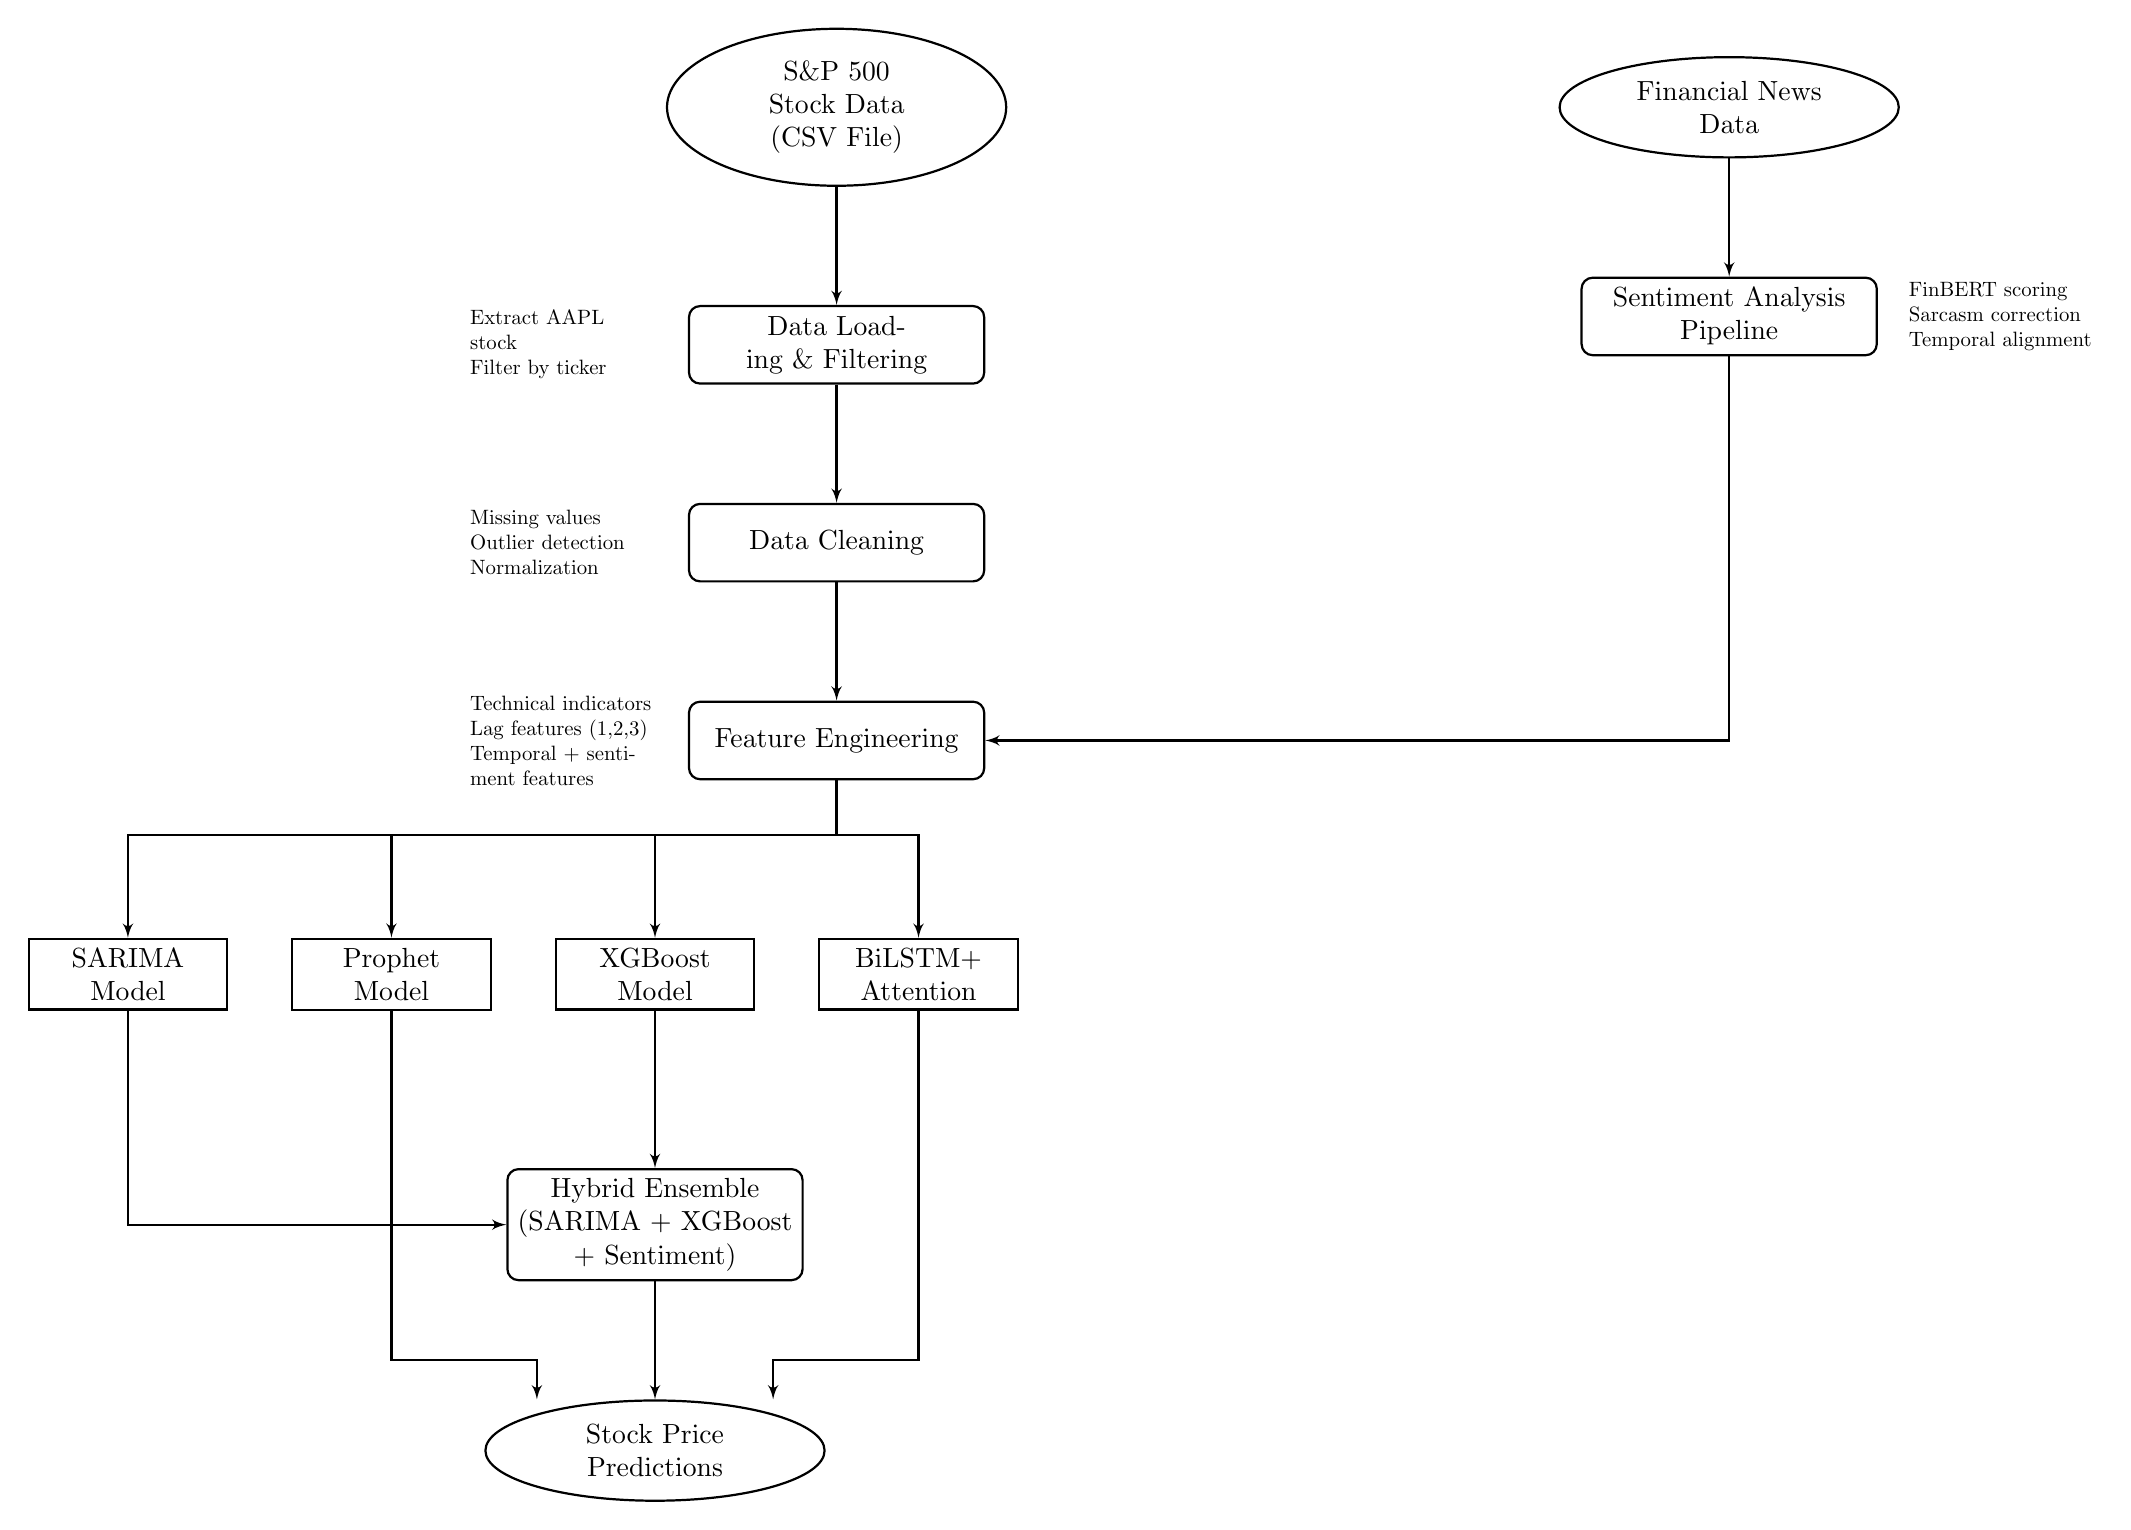
\begin{tikzpicture}[
        node distance=2cm,
        auto,
        block/.style={rectangle, draw, fill=white, text width=10em, text centered, rounded corners, minimum height=2.8em, line width=0.8pt},
        datablock/.style={rectangle, draw, fill=white, text width=7em, text centered, minimum height=2.5em, line width=0.8pt},
        modelblock/.style={rectangle, draw, fill=white, text width=6.5em, text centered, minimum height=2.5em, line width=0.8pt},
        cloud/.style={draw, ellipse, fill=white, text width=8em, text centered, minimum height=2.5em, line width=0.8pt},
        line/.style={draw, -latex', line width=0.8pt},
        annotation/.style={text width=9em, scale=0.75, align=left}
    ]
    
    % Data Input Layer
    \node [cloud] (csv) {S\&P 500 Stock Data\\(CSV File)};
    \node [cloud, right=7cm of csv] (news) {Financial News\\Data};
    
    % Price Preprocessing Path
    \node [block, below=1.5cm of csv] (load) {Data Loading \& Filtering};
    \node [annotation, left=0.3cm of load] {Extract AAPL stock\\Filter by ticker};
    
    \node [block, below=1.5cm of load] (clean) {Data Cleaning};
    \node [annotation, left=0.3cm of clean] {Missing values\\Outlier detection\\Normalization};
    
    % Sentiment Pipeline Path
    \node [block, below=1.5cm of news] (sentpipe) {Sentiment Analysis\\Pipeline};
    \node [annotation, right=0.3cm of sentpipe] {FinBERT scoring\\Sarcasm correction\\Temporal alignment};
    
    % Feature Engineering Layer
    \node [block, below=1.5cm of clean] (features) {Feature Engineering};
    \node [annotation, left=0.3cm of features] {Technical indicators\\Lag features (1,2,3)\\Temporal + sentiment features};
    
    % Model Layer (Horizontal arrangement)
    \node [modelblock, below=2cm of features, xshift=-9cm] (sarima) {SARIMA\\Model};
    \node [modelblock, right=0.8cm of sarima] (prophet) {Prophet\\Model};
    \node [modelblock, right=0.8cm of prophet] (xgb) {XGBoost\\Model};
    \node [modelblock, right=0.8cm of xgb] (bilstm) {BiLSTM+\\Attention};
    
    % Hybrid Ensemble Layer
    \node [block, below=2cm of xgb] (hybrid) {Hybrid Ensemble\\(SARIMA + XGBoost\\+ Sentiment)};
    
    % Output Layer
    \node [cloud, below=1.5cm of hybrid] (output) {Stock Price\\Predictions};
    
    % Connections - Vertical flow
    \path [line] (csv) -- (load);
    \path [line] (news) -- (sentpipe);
    \path [line] (load) -- (clean);
    \path [line] (clean) -- (features);
    \path [line] (sentpipe) |- (features);
    
    % Connections - Features to models
    \path [line] (features) -- ++(0,-1.2) -| (sarima);
    \path [line] (features) -- ++(0,-1.2) -| (prophet);
    \path [line] (features) -- ++(0,-1.2) -| (xgb);
    \path [line] (features) -- ++(0,-1.2) -| (bilstm);
    
    % Connections - Models to hybrid/output
    \path [line] (sarima) |- (hybrid);
    \path [line] (xgb) -- (hybrid);
    
    % Direct outputs from Prophet and BiLSTM
    \path [line] (prophet) |- ($(output.north) + (-1.5,0.5)$) -- ($(output.north) + (-1.5,0)$);
    \path [line] (bilstm) |- ($(output.north) + (1.5,0.5)$) -- ($(output.north) + (1.5,0)$);
    
    % Hybrid to output
    \path [line] (hybrid) -- (output);
    
    \end{tikzpicture}
    \caption{Complete System Architecture for Sentiment-Augmented Hybrid Stock Prediction}
    \label{fig:system_architecture}
\end{figure}

The architecture consists of seven primary components:

\begin{enumerate}
    \item \textbf{Data Source}: Historical S\&P 500 stock data from Yahoo Finance API and financial news articles from multiple sources
    \item \textbf{Data Collection \& Preprocessing}: Data cleaning, missing value handling, and train-test splitting
    \item \textbf{Feature Engineering}: Creation of technical indicators, temporal features, and lag variables
    \item \textbf{Sentiment Analysis Pipeline}: Domain-adapted FinBERT sentiment scoring with dual-head sarcasm correction, temporal alignment, and confidence-weighted aggregation
    \item \textbf{Model Development}: Implementation of multiple prediction models (SARIMA, Prophet, XGBoost, BiLSTM+Attention)
    \item \textbf{Hybrid Ensemble}: Combination of SARIMA for trend capture and XGBoost for sentiment-augmented residual learning
    \item \textbf{Prediction Output}: Price forecasts with model comparison and evaluation metrics
\end{enumerate}

Such a multi-model strategy enables us to use the advantages of each methodology and counterbalance the weakness of the other. The integration of a dedicated sentiment analysis pipeline provides the system with information about exogenous market-moving events that price-only features cannot capture.

\subsection{Data Collection and Preprocessing}

\subsubsection{Data Source and Characteristics}

We utilize the \texttt{yfinance} Python library to retrieve historical stock data for S\&P 500 constituent companies. For each stock, we collect:

\begin{itemize}
    \item \textbf{OHLCV Data}: Open, High, Low, Close prices, and trading Volume
    \item \textbf{Temporal Range}: Multi-year historical data to capture various market conditions
    \item \textbf{Frequency}: Daily stock prices with timestamps
\end{itemize}

The raw data has the following major attributes:
\begin{itemize}
    \item \texttt{Date}: Trading date (index)
    \item \texttt{Open}: Opening price for the trading day
    \item \texttt{High}: Highest price during the trading day
    \item \texttt{Low}: Lowest price during the trading day
    \item \texttt{Close}: Closing price (primary target variable)
    \item \texttt{Volume}: Number of shares traded
    \item \texttt{Adj Close}: Adjusted closing price accounting for corporate actions
\end{itemize}

\subsubsection{Data Cleaning}

There are some vital steps that our data preprocessing pipeline realizes:

\textbf{Missing Value Handling:}
There is a high chance of missing data in financial time-series data because of market holidays, suspension of trading, or data collection mistakes. We employ:
\begin{itemize}
    \item \textbf{Forward Fill}: For single-day gaps, propagate the last available value
    \item \textbf{Interpolation}: For multi-day gaps, apply linear interpolation to maintain smooth transitions
    \item \textbf{Removal}: Discard stocks with excessive missing data ($>$5\% of total observations)
\end{itemize}

\textbf{Outlier Detection and Treatment:}
Radical price changes may cause model training to be inaccurate. We implement:
\begin{equation}
\text{Outlier} = |x_t - \mu| > 3\sigma
\end{equation}
where $\mu$ represents the rolling mean and $\sigma$ represents the rolling standard deviation over a 20-day window.

\textbf{Normalization:}
In order to achieve a numerically stable model convergence we use Min-Max scaling:
\begin{equation}
x_{\text{scaled}} = \frac{x - x_{\min}}{x_{\max} - x_{\min}}
\end{equation}

\subsubsection{News Data Collection}

Financial news articles are collected from publicly available sources to serve as input for the sentiment analysis pipeline. Sources include Yahoo Finance News, Reuters financial RSS feeds, and the Financial Modeling Prep news API. For each article, we collect the following data fields:

\begin{itemize}
    \item \textbf{Headline}: Title of the article
    \item \textbf{Body}: Full article text where available; headline-only for paywalled sources
    \item \textbf{Publication Timestamp}: Exact datetime of publication in UTC
    \item \textbf{Source}: Publisher identifier (e.g., Reuters, Bloomberg, Yahoo Finance)
    \item \textbf{Ticker Mention}: Binary indicator of whether the article explicitly mentions the target stock ticker (e.g., AAPL)
\end{itemize}

The news corpus spans the same temporal range as the price data (2010--2025). Article volume varies considerably over time: high-profile earnings announcements or market-moving events may generate dozens of articles per day, while quiet trading periods may produce none. This variation is explicitly captured through normalized news volume features in the sentiment pipeline. Articles are stored with their original UTC timestamps to enable the principled temporal alignment procedure described in Section~\ref{sec:sentiment_pipeline}.

\subsubsection{Train-Test Split}

We use a temporal split strategy in order to preserve the sequence of time-series information:
\begin{itemize}
    \item \textbf{Training Set}: First 80\% of the chronological data
    \item \textbf{Testing Set}: Final 20\% for out-of-sample evaluation
    \item \textbf{Validation}: Time-series cross-validation with expanding window
\end{itemize}

This will eliminate data leakage and allow realistic evaluation which is a realistic representation of actual trading situations where the future data is unknown.

\subsection{Feature Engineering}

The so-called feature engineering is where the domain knowledge is coded to the model. The features we implement generate three classes of features that profiled various facets of marketing behavior.

\subsubsection{Technical Indicators}

Technical analysis indicators are used to measure momentum, trend, volatility and volume. Some of the indicators that we apply are as follows with the help of the Python library of technical analysis:

\textbf{1. Moving Average Convergence Divergence (MACD):}
\begin{align}
\text{MACD} &= \text{EMA}_{12}(\text{Close}) - \text{EMA}_{26}(\text{Close}) \\
\text{Signal Line} &= \text{EMA}_9(\text{MACD}) \\
\text{MACD Histogram} &= \text{MACD} - \text{Signal Line}
\end{align}

MACD shows the direction of the trend and momentum through comparisons of the short-term average and the long-term average which are exponential moving averages.

\textbf{2. Relative Strength Index (RSI):}
\begin{equation}
\text{RSI} = 100 - \frac{100}{1 + \frac{\text{Avg Gain}_{14}}{\text{Avg Loss}_{14}}}
\end{equation}

RSI is a momentum scale ranging between 0 and 100, where scores of above 70 signal overbought markets and those of below 30 signal oversold markets.

\textbf{3. Bollinger Bands:}
\begin{align}
\text{Middle Band} &= \text{SMA}_{20}(\text{Close}) \\
\text{Upper Band} &= \text{Middle Band} + 2 \times \sigma_{20} \\
\text{Lower Band} &= \text{Middle Band} - 2 \times \sigma_{20}
\end{align}

Bollinger Bands are used to gauge the price volatility based on the 20 days moving average.

\textbf{4. Simple Moving Averages (SMA):}
\begin{equation}
\text{SMA}_n = \frac{1}{n} \sum_{i=0}^{n-1} \text{Close}_{t-i}
\end{equation}

We calculate SMAs for multiple windows ($n = 5, 10, 20, 50, 200$) to capture different trend timescales.

\textbf{5. Exponential Moving Average (EMA):}
\begin{align}
\text{EMA}_t &= \alpha \cdot \text{Close}_t + (1-\alpha) \cdot \text{EMA}_{t-1} \\
\text{where } \alpha &= \frac{2}{n+1}
\end{align}

EMA also places more emphasis on the current prices; hence it is more sensitive to new information than SMA.

\textbf{Additional Technical Indicators:}
\begin{itemize}
    \item \textbf{Stochastic Oscillator}: Measures momentum by comparing closing price to price range
    \item \textbf{Average True Range (ATR)}: Quantifies volatility
    \item \textbf{On-Balance Volume (OBV)}: Cumulative volume indicator for price trend confirmation
    \item \textbf{Commodity Channel Index (CCI)}: Identifies cyclical trends
\end{itemize}

\subsubsection{Temporal Features}

There are high calendar effects in market behavior. We derive time characteristics to reflect such patterns:

\begin{itemize}
    \item \textbf{Day of Week}: One-hot encoded (Monday=0, ..., Friday=4)
    \item \textbf{Month}: One-hot encoded (January=1, ..., December=12)
    \item \textbf{Quarter}: Business quarters (Q1, Q2, Q3, Q4)
    \item \textbf{Is Month End}: Binary indicator for month-end trading effects
    \item \textbf{Is Quarter End}: Binary indicator for quarter-end rebalancing
\end{itemize}

These features enable models to learn the ``January effect,'' ``weekend effect,'' and other calendar-based anomalies documented in financial literature.

\subsubsection{Lag Features}

Time-series prediction is based on autoregressive trends. The lag features are formed based on the closing price:

\begin{equation}
\text{Lag}_k = \text{Close}_{t-k} \quad \text{for } k \in \{1, 2, 3, 5, 10\}
\end{equation}

Such characteristics enable machine learning reasons to explicitly express temporal dependencies without necessitating recurrent designs.

\subsubsection{Feature Selection and Dimensionality}

Once we have feature engineered, we have about 25--30 price-derived features in our data. With the addition of 8 sentiment features (described in Section~\ref{sec:sentiment_features}), the total feature space expands to approximately $d_p + 8 \approx 33$--$38$ dimensions. In order to avoid multicollinearity and overfitting:

\begin{itemize}
    \item \textbf{Correlation Analysis}: Remove features with pairwise correlation $> 0.95$
    \item \textbf{Feature Importance}: Use XGBoost feature importance (ranked by gain) to identify top predictive features
    \item \textbf{Domain Filtering}: Retain features with established financial theory support
    \item \textbf{Variance Inflation Factor (VIF)}: Remove features with VIF $> 10$ to control multicollinearity in the expanded feature space
\end{itemize}

\subsubsection{Sentiment Analysis Pipeline}
\label{sec:sentiment_pipeline}

The sentiment analysis pipeline transforms raw financial news articles into structured, quantitative sentiment signals suitable for integration into the prediction model. The pipeline addresses the critical gaps identified in the literature review---sarcasm detection, tokenization drift, domain sensitivity, temporal alignment, and uncertainty quantification---through a four-stage process. Figure~\ref{fig:sentiment_pipeline} illustrates the complete end-to-end data flow from raw news articles to the final sentiment feature vector.

\begin{figure}[htbp]
    \centering
    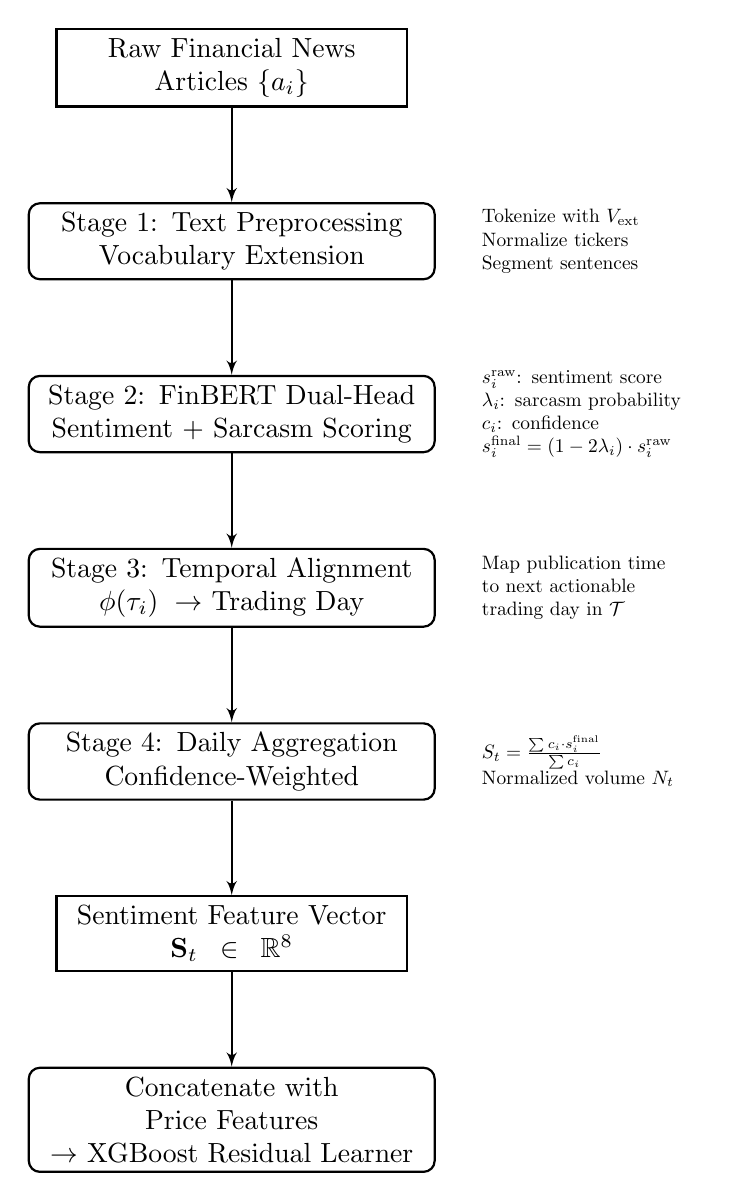
\begin{tikzpicture}[
        node distance=1.2cm,
        process/.style={rectangle, draw, fill=white, text width=14em, text centered, rounded corners, minimum height=2.5em, line width=0.8pt},
        data/.style={rectangle, draw, fill=white, text width=12em, text centered, minimum height=2.2em, line width=0.8pt},
        arrow/.style={draw, -latex', line width=0.8pt},
        note/.style={text width=11em, scale=0.7, align=left}
    ]
    
    \node [data] (input) {Raw Financial News\\Articles $\{a_i\}$};
    
    \node [process, below=of input] (preproc) {Stage 1: Text Preprocessing\\Vocabulary Extension};
    \node [note, right=0.5cm of preproc] {Tokenize with $V_{\text{ext}}$\\Normalize tickers\\Segment sentences};
    
    \node [process, below=of preproc] (finbert) {Stage 2: FinBERT Dual-Head\\Sentiment + Sarcasm Scoring};
    \node [note, right=0.5cm of finbert] {$s_i^{\text{raw}}$: sentiment score\\$\lambda_i$: sarcasm probability\\$c_i$: confidence\\$s_i^{\text{final}} = (1-2\lambda_i) \cdot s_i^{\text{raw}}$};
    
    \node [process, below=of finbert] (temporal) {Stage 3: Temporal Alignment\\$\phi(\tau_i) \to$ Trading Day};
    \node [note, right=0.5cm of temporal] {Map publication time\\to next actionable\\trading day in $\mathcal{T}$};
    
    \node [process, below=of temporal] (aggregate) {Stage 4: Daily Aggregation\\Confidence-Weighted};
    \node [note, right=0.5cm of aggregate] {$S_t = \frac{\sum c_i \cdot s_i^{\text{final}}}{\sum c_i}$\\Normalized volume $N_t$};
    
    \node [data, below=of aggregate] (features) {Sentiment Feature Vector\\$\mathbf{S}_t \in \mathbb{R}^8$};
    
    \node [process, below=of features] (xgboost) {Concatenate with Price Features\\$\to$ XGBoost Residual Learner};
    
    \path [arrow] (input) -- (preproc);
    \path [arrow] (preproc) -- (finbert);
    \path [arrow] (finbert) -- (temporal);
    \path [arrow] (temporal) -- (aggregate);
    \path [arrow] (aggregate) -- (features);
    \path [arrow] (features) -- (xgboost);
    
    \end{tikzpicture}
    \caption{Sentiment Analysis Pipeline: End-to-End Data Flow from Raw News to XGBoost Integration}
    \label{fig:sentiment_pipeline}
\end{figure}

\textbf{Base Model: FinBERT}

The sentiment scoring component is built on FinBERT, a domain-adapted variant of BERT (Bidirectional Encoder Representations from Transformers). BERT is a transformer-based neural network that uses multi-head self-attention to learn contextualized word representations. Unlike static word embeddings that assign a fixed vector to each word regardless of context, BERT produces context-dependent representations: the word ``crash'' receives a different embedding in ``stock market crash'' than in ``application crash.''

FinBERT inherits BERT's 12-layer, 768-dimensional transformer encoder architecture (approximately 110 million parameters) and is further pre-trained on a large corpus of financial communications including financial news articles, earnings call transcripts, and analyst reports. This domain-specific pre-training allows FinBERT to correctly interpret financial expressions that general-purpose BERT misclassifies---for example, FinBERT understands that ``the company beat earnings expectations'' carries positive sentiment, whereas general BERT may be uncertain about the polarity of ``beat'' in a financial context.

The sentiment classification head maps the \texttt{[CLS]} token embedding---a 768-dimensional vector that summarizes the entire input sequence---to a three-class probability distribution (Positive, Negative, Neutral) via a fully connected layer and softmax activation. In our dual-head architecture, a second fully connected layer branches from the same \texttt{[CLS]} embedding to produce a binary sarcasm probability via sigmoid activation. Both heads share the same transformer backbone, so financial language understanding learned by the sentiment head also benefits sarcasm detection.

\textbf{Training Data and Fine-Tuning Procedure}

The dual-head model is fine-tuned on two labeled datasets:
\begin{enumerate}
    \item \textbf{Sentiment Labels}: The Financial Phrasebank dataset provides approximately 4,840 English financial news sentences labeled by 16 financial experts as Positive, Negative, or Neutral. We use the subset with $\geq 75\%$ annotator agreement to ensure label quality.
    \item \textbf{Sarcasm Labels}: A curated financial sarcasm dataset containing approximately 3,000 labeled examples, constructed by collecting financial headlines with confirmed sarcastic intent (marked by expert annotators) and augmenting with non-sarcastic financial headlines as negative examples.
\end{enumerate}

Fine-tuning proceeds in two phases to prevent catastrophic forgetting of the pre-trained representations:
\begin{enumerate}
    \item \textbf{Phase 1 --- Frozen Backbone}: The FinBERT transformer weights are frozen. Only the two classification heads (sentiment and sarcasm) are trained for 5 epochs with a learning rate of $2 \times 10^{-4}$. This allows the heads to initialize without corrupting the pre-trained language representations.
    \item \textbf{Phase 2 --- Joint Fine-Tuning}: All model weights (backbone + both heads) are unfrozen, and the entire model is trained end-to-end for 3 additional epochs with a reduced learning rate of $2 \times 10^{-5}$. The combined training objective is:
    \begin{equation}
    \mathcal{L}_{\text{total}} = \alpha \cdot \mathcal{L}_{\text{sentiment}} + (1 - \alpha) \cdot \mathcal{L}_{\text{sarcasm}}
    \end{equation}
    where $\alpha = 0.7$ prioritizes the primary sentiment task, $\mathcal{L}_{\text{sentiment}}$ is categorical cross-entropy over three classes, and $\mathcal{L}_{\text{sarcasm}}$ is binary cross-entropy. Training uses the AdamW optimizer with a batch size of 32 and linear learning rate warmup over the first 10\% of training steps.
\end{enumerate}

The four processing stages of the pipeline are described below.

\textbf{Stage 1: Text Preprocessing with Vocabulary Extension}

Before sentiment scoring, each article undergoes domain-aware preprocessing. The standard FinBERT tokenizer is extended with a custom financial vocabulary containing common ticker symbols, financial ratios, and regulatory terms to address the tokenization drift gap. Given the original FinBERT vocabulary $V_{\text{FinBERT}}$, the extended vocabulary is:
\begin{equation}
V_{\text{ext}} = V_{\text{FinBERT}} \cup V_{\text{fin}}
\end{equation}

where $V_{\text{fin}}$ is a curated set of financial domain tokens including ticker symbols, financial ratios (P/E, EV/EBITDA), and regulatory terminology (Form 10-K, material adverse change). Ticker symbols in the format \$TICKER are normalized to a canonical form TICKER\_REF to prevent subword fragmentation. URLs, HTML entities, and boilerplate disclosure text are removed, while numerical values are retained as they carry information about financial magnitudes.

Long articles are segmented into individual sentences, and each sentence is scored independently before aggregation at the document level. This preserves local sentiment nuance that document-level scoring would otherwise lose.

\textbf{Stage 2: Dual-Head Sentiment Scoring}

The core of the pipeline is a dual-head classification model built on the FinBERT transformer backbone. The model has two output heads sharing the same encoder:
\begin{itemize}
    \item \textbf{Head 1 (Sentiment Head)}: A three-class classifier (Positive, Negative, Neutral) producing a probability distribution $P_{\text{sent}}(c \mid a_i)$ for article $a_i$.
    \item \textbf{Head 2 (Sarcasm Head)}: A binary classifier producing the probability of sarcasm $P_{\text{sarc}}(a_i)$.
\end{itemize}

The raw sentiment score is converted to a continuous scale:
\begin{equation}
s_i^{\text{raw}} = P_{\text{sent}}(\text{Positive} \mid a_i) - P_{\text{sent}}(\text{Negative} \mid a_i) \in [-1, 1]
\end{equation}

The sarcasm-corrected sentiment score inverts the raw score in proportion to the estimated probability of sarcasm:
\begin{equation}
s_i^{\text{final}} = (1 - 2\lambda_i) \cdot s_i^{\text{raw}}
\end{equation}

where $\lambda_i = P_{\text{sarc}}(a_i) \in [0, 1]$. When $\lambda_i = 0$ (no sarcasm), the raw score is preserved; when $\lambda_i = 1$ (definite sarcasm), the sentiment polarity is fully inverted. The confidence of the prediction is defined as:
\begin{equation}
c_i = \max_{k \in \{\text{Pos}, \text{Neg}, \text{Neu}\}} P_{\text{sent}}(k \mid a_i) \in \left[\tfrac{1}{3}, 1\right]
\end{equation}

\textbf{Stage 3: Temporal Alignment}

Let $\tau_i$ denote the UTC publication timestamp of article $a_i$. The trading-day assignment function $\phi(\tau_i)$ maps each article to the appropriate trading day:
\begin{equation}
\phi(\tau_i) = \min\{t \in \mathcal{T} : \text{MarketOpen}(t) > \tau_i\}
\end{equation}

where $\mathcal{T}$ is the set of valid NYSE trading days. This formal assignment ensures:
\begin{itemize}
    \item Articles published during or after market hours on day $t$ are assigned to the next trading day $t+1$.
    \item Articles published after market close on Friday are assigned to Monday (or the next valid trading day if Monday is a holiday).
    \item No future information leaks into the training set.
\end{itemize}

\textbf{Stage 4: Daily Sentiment Aggregation}

For trading day $t$, let $\mathcal{A}_t = \{a_i : \phi(\tau_i) = t\}$ be the set of articles assigned to that day. The confidence-weighted daily sentiment score is:
\begin{equation}
S_t = \frac{\sum_{a_i \in \mathcal{A}_t} c_i \cdot s_i^{\text{final}}}{\sum_{a_i \in \mathcal{A}_t} c_i}
\end{equation}

If $\mathcal{A}_t = \emptyset$ (no news on trading day $t$), then $S_t = 0$ (neutral). The daily news volume, normalized over the dataset, is:
\begin{equation}
N_t = \frac{|\mathcal{A}_t| - \mu_N}{\sigma_N}
\end{equation}

where $\mu_N$ and $\sigma_N$ are the mean and standard deviation of daily article counts over the training period.

\textbf{End-to-End Daily Processing Loop}

The complete pipeline operates as a daily batch process executed after market close. For each trading day $t$, the system performs the following sequence:

\begin{enumerate}
    \item \textbf{Collect}: Retrieve all news articles $\{a_i\}$ published since the last processing run from the configured news sources (Yahoo Finance, Reuters RSS, Financial Modeling Prep API).
    \item \textbf{Preprocess}: For each article $a_i$, apply vocabulary-extended tokenization, ticker normalization, boilerplate removal, and sentence segmentation (Stage~1).
    \item \textbf{Score}: Pass each preprocessed sentence through the dual-head FinBERT model. The sentiment head produces the raw score $s_i^{\text{raw}}$ and confidence $c_i$; the sarcasm head produces $\lambda_i$. Compute the sarcasm-corrected score $s_i^{\text{final}} = (1 - 2\lambda_i) \cdot s_i^{\text{raw}}$ (Stage~2). For multi-sentence articles, aggregate sentence-level scores to a single document-level score weighted by sentence confidence.
    \item \textbf{Align}: Apply the temporal assignment function $\phi(\tau_i)$ to each article's UTC timestamp to determine the correct target trading day. Articles published after today's market close are assigned to the next trading day (Stage~3).
    \item \textbf{Aggregate}: For the target trading day $t$, compute the confidence-weighted daily sentiment $S_t$ and the normalized news volume $N_t$ from all articles in $\mathcal{A}_t$. If $\mathcal{A}_t = \emptyset$, set $S_t = 0$ and flag $I_t^{\text{no\_news}} = 1$ (Stage~4).
    \item \textbf{Derive Features}: Using the aggregated $S_t$ and the historical sentiment values $S_{t-1}, S_{t-2}, S_{t-3}$, compute the full 8-dimensional sentiment feature vector $\mathbf{S}_t = [S_t, \Delta S_t, \sigma_{S,t}, N_t, D_t, S_{t-1}, S_{t-2}, S_{t-3}]$.
    \item \textbf{Integrate}: Concatenate $\mathbf{S}_t$ with the price-derived feature vector $\mathbf{X}_t^{\text{price}}$ to form $\mathbf{X}_t^{\text{ext}}$, which is passed to the XGBoost residual learner alongside the SARIMA baseline prediction.
\end{enumerate}

This daily loop ensures strict temporal causality: sentiment features for trading day $t$ are computed exclusively from articles published before day $t$'s market open, preventing any form of information leakage. The entire processing cycle (collection, scoring, feature computation) takes approximately 2--5 minutes on standard CPU hardware depending on news volume, making it feasible as an overnight batch process.

\subsubsection{Sentiment Feature Engineering}
\label{sec:sentiment_features}

From the raw daily sentiment signal $S_t$ and the news volume $N_t$ produced by the sentiment pipeline, we derive a structured set of eight features that capture different aspects of the sentiment dynamics.

\textbf{1. Daily Aggregated Sentiment ($S_t$):}
The confidence-weighted, sarcasm-corrected daily sentiment score as defined in Section~\ref{sec:sentiment_pipeline}.

\textbf{2. Sentiment Momentum ($\Delta S_t$):}
\begin{equation}
\Delta S_t = S_t - S_{t-1}
\end{equation}
Captures sudden shifts in news sentiment that may precede price movements.

\textbf{3. Rolling Sentiment Volatility ($\sigma_{S,t}$):}
\begin{equation}
\sigma_{S,t} = \sqrt{\frac{1}{k} \sum_{j=0}^{k-1} \left(S_{t-j} - \bar{S}_{t,k}\right)^2}
\end{equation}
where $k = 5$ (one trading week) and $\bar{S}_{t,k} = \frac{1}{k}\sum_{j=0}^{k-1} S_{t-j}$. High sentiment volatility indicates an unstable news environment and may signal increased price volatility.

\textbf{4. Normalized News Volume ($N_t$):}
Z-score normalized daily article count, capturing the intensity of news coverage. Abnormally high news volume often accompanies significant price-moving events.

\textbf{5. Sentiment-Price Divergence ($D_t$):}
\begin{equation}
D_t = S_{t-1} - \text{sign}\left(\text{Close}_{t-1} - \text{Close}_{t-2}\right)
\end{equation}
Measures the alignment between the prior day's sentiment and price movement. A large positive divergence (positive sentiment but negative return) may signal a mean-reversion opportunity.

\textbf{6--8. Lagged Sentiment Features ($S_{t-1}, S_{t-2}, S_{t-3}$):}
\begin{equation}
S_{t-k} \quad \text{for } k \in \{1, 2, 3\}
\end{equation}
Capture the delayed reaction of prices to news sentiment over a three-day horizon.

\vspace{0.5cm}
\noindent The full sentiment feature vector for day $t$ is:
\begin{equation}
\mathbf{S}_t = \left[S_t,\; \Delta S_t,\; \sigma_{S,t},\; N_t,\; D_t,\; S_{t-1},\; S_{t-2},\; S_{t-3}\right] \in \mathbb{R}^8
\end{equation}

This structured representation provides the downstream XGBoost model with richer and more reliable sentiment signals than raw point estimates, addressing the uncertainty quantification gap identified in the literature review.

\subsection{Model Development}

There are five types of prediction models that we apply and each of them reflects various features of the stock prices dynamics.

\subsubsection{SARIMA Model}

\textbf{Model Overview:}
Seasonal AutoRegressive Integrated Moving Average (SARIMA) extends ARIMA by explicitly modeling seasonal patterns. The model is specified as SARIMA$(p, d, q) \times (P, D, Q)_s$ where:

\begin{itemize}
    \item $(p, d, q)$: Non-seasonal AR order, differencing, MA order
    \item $(P, D, Q)$: Seasonal AR order, differencing, MA order
    \item $s$: Seasonality period (e.g., 5 for weekly patterns in daily data)
\end{itemize}

\textbf{Mathematical Formulation:}
\begin{equation}
\phi_p(B)\Phi_P(B^s)(1-B)^d(1-B^s)^D y_t = \theta_q(B)\Theta_Q(B^s)\epsilon_t
\end{equation}

where:
\begin{itemize}
    \item $B$: Backward shift operator ($B^k y_t = y_{t-k}$)
    \item $\phi_p(B)$: Non-seasonal AR polynomial
    \item $\Phi_P(B^s)$: Seasonal AR polynomial
    \item $\theta_q(B)$: Non-seasonal MA polynomial
    \item $\Theta_Q(B^s)$: Seasonal MA polynomial
    \item $\epsilon_t$: White noise error term
\end{itemize}

\textbf{Implementation Details:}
We use the \texttt{pmdarima} library's \texttt{auto\_arima} function for automated parameter selection:

\begin{itemize}
    \item \textbf{Order Selection}: Auto-ARIMA searches over parameter space to minimize AIC/BIC
    \item \textbf{Stationarity Testing}: Augmented Dickey-Fuller test for unit roots
    \item \textbf{Seasonality Detection}: Automatic identification of seasonal patterns
    \item \textbf{Final Configuration}: SARIMA$(0,1,0) \times (0,0,0)_{[5]}$ (identified by auto-fitting)
\end{itemize}

\textbf{Training Process:}
\begin{enumerate}
    \item Test for stationarity using ADF test
    \item Apply differencing if necessary to achieve stationarity
    \item Fit SARIMA model using maximum likelihood estimation
    \item Validate residuals for white noise properties (Ljung-Box test)
    \item Generate forecasts for test period
\end{enumerate}

\subsubsection{Prophet Model}

\textbf{Model Overview:}
Prophet, developed by Facebook (Meta), employs an additive model framework particularly suited for business time-series with strong seasonal effects and multiple trend changes.

\textbf{Mathematical Formulation:}
\begin{equation}
y(t) = g(t) + s(t) + h(t) + \epsilon_t
\end{equation}

where:
\begin{itemize}
    \item $g(t)$: Piecewise linear or logistic growth trend
    \item $s(t)$: Periodic component (daily, weekly, yearly seasonality)
    \item $h(t)$: Holiday/event effects
    \item $\epsilon_t$: Idiosyncratic error term
\end{itemize}

\textbf{Trend Component:}
Prophet determines non-linear trends with the help of changepoint:
\begin{equation}
g(t) = (k + \mathbf{a}(t)^T\delta)t + (m + \mathbf{a}(t)^T\gamma)
\end{equation}

where the value of delta is rate changes at changepoints that are automatically identified.

\textbf{Seasonality Component:}
Fourier series is used to model seasonality:
\begin{equation}
s(t) = \sum_{n=1}^{N} \left( a_n \cos\left(\frac{2\pi nt}{P}\right) + b_n \sin\left(\frac{2\pi nt}{P}\right) \right)
\end{equation}

where $P$ is the period (365.25 for yearly, 7 for weekly).

\textbf{Implementation Details:}
\begin{itemize}
    \item \textbf{Library}: \texttt{fbprophet} Python package
    \item \textbf{Changepoint Prior}: 0.05 (controls flexibility of trend)
    \item \textbf{Seasonality Mode}: Multiplicative (appropriate for percentage changes)
    \item \textbf{Weekly Seasonality}: Enabled to capture weekday effects
    \item \textbf{Uncertainty Intervals}: 95\% prediction intervals via MCMC sampling
\end{itemize}

\subsubsection{XGBoost Model}

\textbf{Model Overview:}
XGBoost (eXtreme Gradient Boosting) is a system that adopts optimized gradient boosting decision trees. Compared to other statistical models, XGBoost is able to automatically formulate non-linear interactions between features and can work effectively with mixed data types.

\textbf{Mathematical Formulation:}
XGBoost creates an additive regression of the weak decision trees learners:
\begin{equation}
\hat{y}_i = \sum_{k=1}^{K} f_k(\mathbf{x}_i), \quad f_k \in \mathcal{F}
\end{equation}

where $\mathcal{F}$ represents the space of regression trees, and each tree $f_k$ is learned to minimize the objective:
\begin{equation}
\mathcal{L}^{(t)} = \sum_{i=1}^{n} l(y_i, \hat{y}_i^{(t-1)} + f_t(\mathbf{x}_i)) + \Omega(f_t)
\end{equation}

The overfitting is avoided by the regularization term:
\begin{equation}
\Omega(f) = \gamma T + \frac{1}{2}\lambda ||\mathbf{w}||^2
\end{equation}

where $T$ is the number of leaves and $\mathbf{w}$ represents leaf weights.

\textbf{Implementation Details:}
\begin{itemize}
    \item \textbf{Library}: \texttt{xgboost} Python package
    \item \textbf{Objective Function}: \texttt{reg:squarederror} (regression)
    \item \textbf{Number of Estimators}: 100 trees
    \item \textbf{Learning Rate}: 0.1 (step size shrinkage)
    \item \textbf{Max Depth}: 5 (maximum tree depth)
    \item \textbf{Subsample}: 0.8 (row sampling ratio)
    \item \textbf{Colsample by Tree}: 0.8 (column sampling ratio)
    \item \textbf{Early Stopping}: Monitor validation RMSE with patience=10
\end{itemize}

\textbf{Feature Set:}
XGBoost makes use of the entire engineered set that consists of:
\begin{itemize}
    \item All technical indicators (MACD, RSI, Bollinger Bands, etc.)
    \item Temporal features (day of week, month, quarter)
    \item Lag features (1, 2, 3, 5, 10 days)
    \item Volume-derived features
\end{itemize}

\textbf{Hyperparameter Optimization:}
We use grid search and time-series cross-validation to optimize hyperparameters in the search space:
\begin{itemize}
    \item Learning rate: $\{0.01, 0.05, 0.1, 0.2\}$
    \item Max depth: $\{3, 5, 7, 10\}$
    \item Number of estimators: $\{50, 100, 200, 300\}$
\end{itemize}

\subsubsection{BiLSTM + Attention Model}

\textbf{Model Overview:}
The Bidirectional Long Short-Term Memory (BiLSTM) networks are coupled with a modification of the attention process in our deep learning architecture. The architecture offers better results than vanilla LSTMs because it takes into account the constraints of processing sequences in both time directions and selectively concentrating on the most informative time steps.

\begin{figure}[htbp]
    \centering
    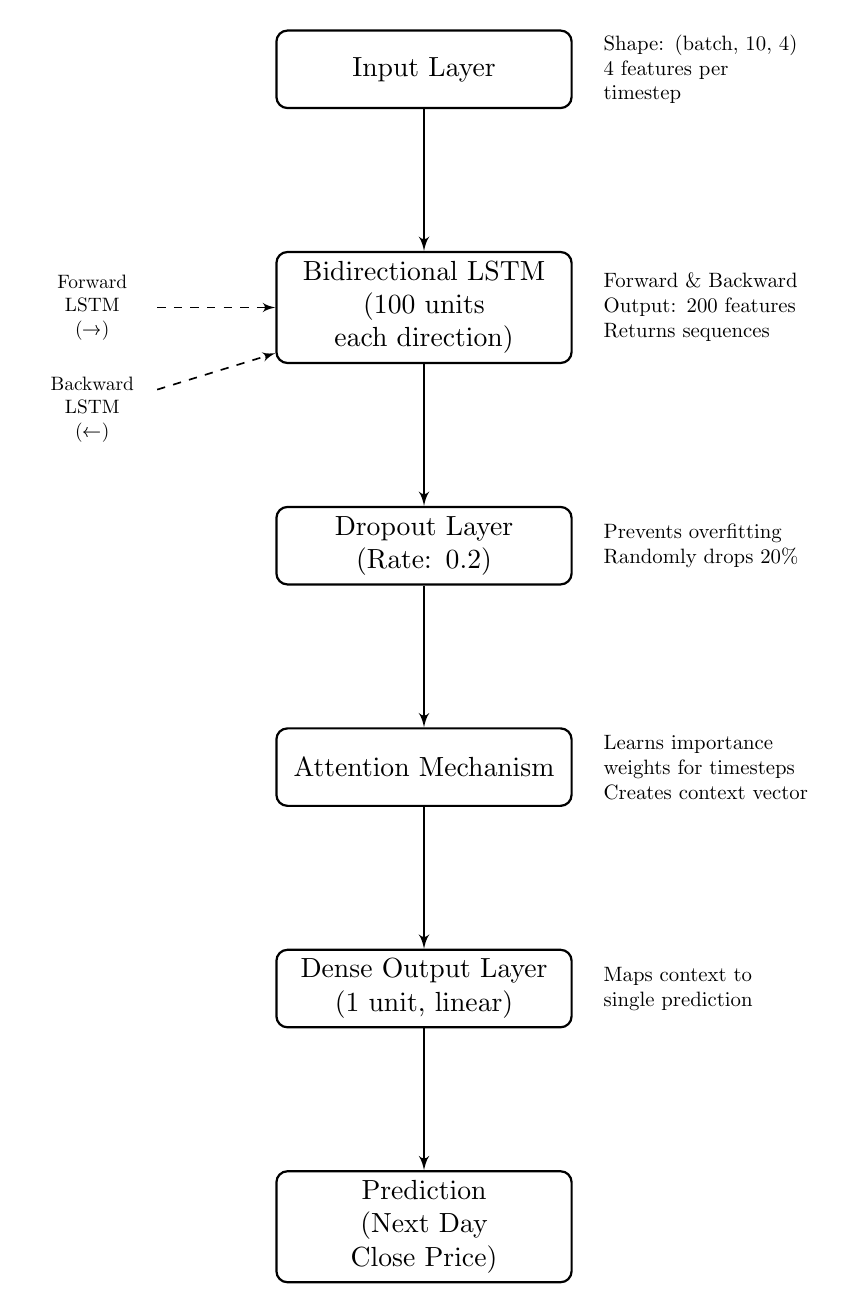
\begin{tikzpicture}[
        node distance=1.8cm,
        auto,
        layer/.style={rectangle, draw, fill=white, text width=10em, text centered, rounded corners, minimum height=2.8em, line width=0.8pt},
        arrow/.style={draw, -latex', line width=0.8pt},
        annotation/.style={text width=10em, scale=0.75, align=left},
        dashedarrow/.style={draw, dashed, -latex', line width=0.6pt}
    ]
    
    % Input Layer
    \node [layer] (input) {Input Layer};
    \node [annotation, right=0.3cm of input] {Shape: (batch, 10, 4)\\4 features per timestep};
    
    % BiLSTM Layer with forward/backward visualization
    \node [layer, below=of input] (bilstm) {Bidirectional LSTM\\(100 units each direction)};
    \node [annotation, right=0.3cm of bilstm] {Forward \& Backward\\Output: 200 features\\Returns sequences};
    
    % Dropout Layer
    \node [layer, below=of bilstm] (dropout) {Dropout Layer\\(Rate: 0.2)};
    \node [annotation, right=0.3cm of dropout] {Prevents overfitting\\Randomly drops 20\%};
    
    % Attention Mechanism
    \node [layer, below=of dropout] (attention) {Attention Mechanism};
    \node [annotation, right=0.3cm of attention] {Learns importance\\weights for timesteps\\Creates context vector};
    
    % Dense Output Layer
    \node [layer, below=of attention] (dense) {Dense Output Layer\\(1 unit, linear)};
    \node [annotation, right=0.3cm of dense] {Maps context to\\single prediction};
    
    % Final Output
    \node [layer, below=of dense] (output) {Prediction\\(Next Day Close Price)};
    
    % Main flow arrows
    \path [arrow] (input) -- (bilstm);
    \path [arrow] (bilstm) -- (dropout);
    \path [arrow] (dropout) -- (attention);
    \path [arrow] (attention) -- (dense);
    \path [arrow] (dense) -- (output);
    
    % Side annotation for BiLSTM showing forward/backward
    \node [left=1.5cm of bilstm, text width=6em, scale=0.7, align=center] (fwd) {Forward\\LSTM\\(→)};
    \node [below=0.3cm of fwd, text width=6em, scale=0.7, align=center] (bwd) {Backward\\LSTM\\(←)};
    \path [dashedarrow] (fwd) -- (bilstm);
    \path [dashedarrow] (bwd) -- (bilstm);
    
    \end{tikzpicture}
    \caption{BiLSTM with Attention Mechanism Architecture}
    \label{fig:bilstm_attention}
\end{figure}

\textbf{Architecture Components:}

\textbf{1. Input Layer:}
\begin{itemize}
    \item \textbf{Shape}: $(\text{batch\_size}, \text{timesteps}, \text{features})$
    \item \textbf{Configuration}: $(None, 10, 4)$ --- 10 historical days, 4 features (Open, High, Low, Close)
\end{itemize}

\textbf{2. Bidirectional LSTM Layer:}

The BiLSTM works off of the input sequence in both directions:
\begin{align}
\overrightarrow{h}_t &= \text{LSTM}_{\text{forward}}(x_t, \overrightarrow{h}_{t-1}) \\
\overleftarrow{h}_t &= \text{LSTM}_{\text{backward}}(x_t, \overleftarrow{h}_{t+1}) \\
h_t &= [\overrightarrow{h}_t; \overleftarrow{h}_t]
\end{align}

Both LSTM cells have gating mechanisms:
\begin{align}
f_t &= \sigma(W_f \cdot [h_{t-1}, x_t] + b_f) \quad \text{(Forget gate)} \\
i_t &= \sigma(W_i \cdot [h_{t-1}, x_t] + b_i) \quad \text{(Input gate)} \\
\tilde{C}_t &= \tanh(W_C \cdot [h_{t-1}, x_t] + b_C) \quad \text{(Candidate values)} \\
C_t &= f_t \odot C_{t-1} + i_t \odot \tilde{C}_t \quad \text{(Cell state)} \\
o_t &= \sigma(W_o \cdot [h_{t-1}, x_t] + b_o) \quad \text{(Output gate)} \\
h_t &= o_t \odot \tanh(C_t) \quad \text{(Hidden state)}
\end{align}

\begin{itemize}
    \item \textbf{Units}: 100 (50 forward + 50 backward)
    \item \textbf{Return Sequences}: True (outputs sequence for attention layer)
    \item \textbf{Activation}: \texttt{tanh} (cell state), \texttt{sigmoid} (gates)
\end{itemize}

\textbf{3. Dropout Layer:}
\begin{itemize}
    \item \textbf{Dropout Rate}: 0.2
    \item \textbf{Purpose}: Prevent overfitting by randomly zeroing 20\% of outputs
\end{itemize}

\textbf{4. Custom Attention Mechanism:}

Our layer of attention is trained to give the weight of various time steps:

\begin{align}
e_t &= \tanh(W_a \cdot h_t + b_a) \quad \text{(Attention scores)} \\
\alpha_t &= \frac{\exp(e_t)}{\sum_{i=1}^{T} \exp(e_i)} \quad \text{(Normalized weights)} \\
c &= \sum_{t=1}^{T} \alpha_t h_t \quad \text{(Context vector)}
\end{align}

where:
\begin{itemize}
    \item $W_a, b_a$: Trainable attention parameters
    \item $\alpha_t$: Attention weights (sum to 1)
    \item $c$: Weighted sum of hidden states (context vector)
\end{itemize}

The attention mechanism helps the model to concentrate on important patterns (e.g. recent volatility spikes, trend reversals) and on less informative periods gives less weight.

\textbf{5. Dense Output Layer:}
\begin{itemize}
    \item \textbf{Units}: 1 (scalar price prediction)
    \item \textbf{Activation}: Linear (for regression)
\end{itemize}

\textbf{Model Compilation:}
\begin{itemize}
    \item \textbf{Optimizer}: Adam with learning rate = 0.001
    \item \textbf{Loss Function}: Mean Squared Error (MSE)
    \item \textbf{Metrics}: MAE, RMSE
\end{itemize}

\textbf{Training Configuration:}
\begin{itemize}
    \item \textbf{Epochs}: 50 with early stopping (patience=10)
    \item \textbf{Batch Size}: 32
    \item \textbf{Validation Split}: 20\% of training data for validation
    \item \textbf{Callbacks}: ModelCheckpoint (save best model), EarlyStopping, ReduceLROnPlateau
\end{itemize}

\textbf{Data Preparation for BiLSTM:}
We take sliding windows on the time series:
\begin{itemize}
    \item \textbf{Sequence Length}: 10 days
    \item \textbf{Prediction Horizon}: 1 day ahead (next closing price)
    \item \textbf{Stride}: 1 day (overlapping windows)
\end{itemize}

For a dataset with $N$ days, we generate $N - 10$ training samples, each containing 10 consecutive days of features and the following day's close price as the target.

\subsubsection{Hybrid SARIMA-XGBoost Model}

\textbf{Model Overview:}
The hybrid model incorporates the complementary power of SARIMA and XGBoost with the help of a two-stage residual learning structure. SARIMA takes in linear trends and seasonality, and XGBoost trains the non-linear residual trends which SARIMA is unable to capture.

\begin{figure}[htbp]
    \centering
    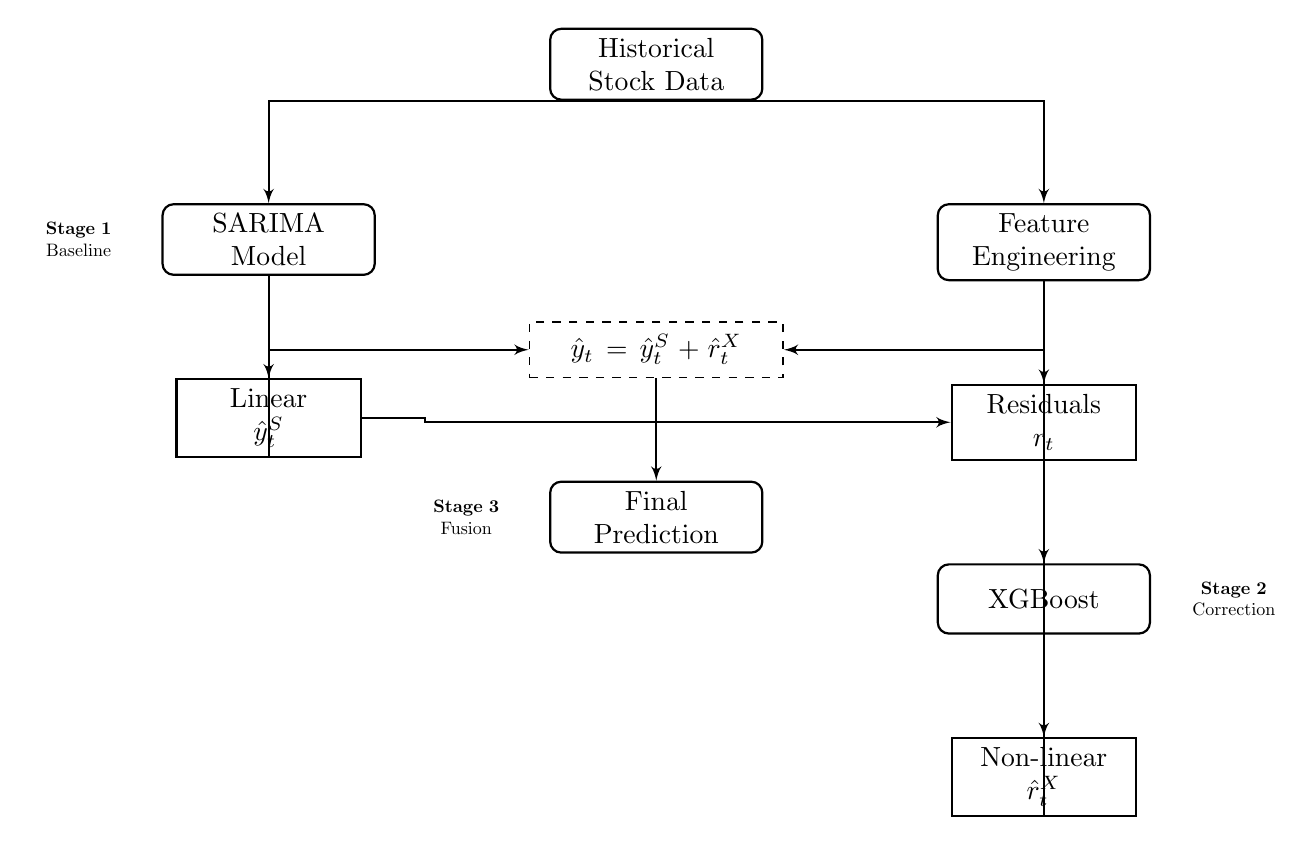
\begin{tikzpicture}[
        node distance=1.3cm and 2.2cm,
        process/.style={rectangle, draw, fill=white, text width=7em, text centered, rounded corners, minimum height=2.5em, line width=0.8pt},
        data/.style={rectangle, draw, fill=white, text width=6em, text centered, minimum height=2.2em, line width=0.8pt},
        equation/.style={rectangle, draw, dashed, fill=white, text width=8.5em, text centered, minimum height=2em, line width=0.6pt},
        arrow/.style={draw, -latex', line width=0.8pt},
        note/.style={text width=5em, scale=0.65, align=center}
    ]
    
    % Main vertical flow
    \node [process] (input) {Historical\\Stock Data};
    
    % Stage 1: SARIMA branch (left)
    \node [process, below left=of input] (sarima) {SARIMA\\Model};
    \node [data, below=of sarima] (linear) {Linear\\$\hat{y}_t^{S}$};
    
    % Stage 2: Feature Engineering & XGBoost branch (right)
    \node [process, below right=of input] (features) {Feature\\Engineering};
    \node [data, below=of features] (residuals) {Residuals\\$r_t$};
    \node [process, below=of residuals] (xgboost) {XGBoost};
    \node [data, below=of xgboost] (nonlinear) {Non-linear\\$\hat{r}_t^{X}$};
    
    % Stage 3: Fusion
    \node [equation, below=2.8cm of input] (fusion) {$\hat{y}_t = \hat{y}_t^{S} + \hat{r}_t^{X}$};
    \node [process, below=of fusion] (output) {Final\\Prediction};
    
    % Connections - using anchor points to avoid overlap
    \path [arrow] (input.south) -| (sarima.north);
    \path [arrow] (input.south) -| (features.north);
    \path [arrow] (sarima) -- (linear);
    \path [arrow] (features) -- (residuals);
    
    % Route from linear to residuals around the diagram
    \path [arrow] (linear.east) -- ++(0.8,0) |- (residuals.west);
    
    \path [arrow] (residuals) -- (xgboost);
    \path [arrow] (xgboost) -- (nonlinear);
    
    % Route to fusion from both sides
    \path [arrow] (linear.south) |- (fusion.west);
    \path [arrow] (nonlinear.south) |- (fusion.east);
    
    \path [arrow] (fusion) -- (output);
    
    % Stage labels - positioned to avoid overlap
    \node [note, left=0.4cm of sarima] {\textbf{Stage 1}\\Baseline};
    \node [note, right=0.4cm of xgboost] {\textbf{Stage 2}\\Correction};
    \node [note, left=0.4cm of output] {\textbf{Stage 3}\\Fusion};
    
    \end{tikzpicture}
    \caption{Hybrid SARIMA-XGBoost Workflow}
    \label{fig:hybrid_workflow}
\end{figure}

\textbf{Hybrid Architecture Rationale:}

Financial time series are a two sided phenomenon:
\begin{equation}
y_t = L_t + N_t + \epsilon_t
\end{equation}

where:
\begin{itemize}
    \item $L_t$: Linear component (trends, seasonality, autocorrelation)
    \item $N_t$: Non-linear component (regime shifts, volatility clustering, feature interactions)
    \item $\epsilon_t$: Random noise
\end{itemize}

SARIMA excels at modeling $L_t$ through its ARMA structure, while XGBoost captures $N_t$ through its decision tree ensemble.

\textbf{Implementation Pipeline:}

\textbf{Stage 1: SARIMA Baseline}
\begin{enumerate}
    \item Train SARIMA$(0,1,0) \times (0,0,0)_{[5]}$ on training data
    \item Generate forecasts: $\hat{y}_t^{\text{SARIMA}}$
    \item Calculate residuals: $r_t = y_t - \hat{y}_t^{\text{SARIMA}}$
\end{enumerate}

\textbf{Stage 2: XGBoost Residual Modeling}
\begin{enumerate}
    \item Engineer features from original data (lag features, technical indicators)
    \item Train XGBoost to predict residuals: $r_t \sim f(\mathbf{X}_t)$
    \item Generate residual predictions: $\hat{r}_t^{\text{XGBoost}}$
\end{enumerate}

\textbf{Stage 3: Hybrid Fusion}
\begin{equation}
\hat{y}_t^{\text{Hybrid}} = \hat{y}_t^{\text{SARIMA}} + \hat{r}_t^{\text{XGBoost}}
\end{equation}

\textbf{Mathematical Justification:}

Assuming that SARIMA is able to capture the linear component, the residual of SARIMA will only have the non-linear component and noise:
\begin{equation}
r_t = y_t - \hat{y}_t^{\text{SARIMA}} \approx N_t + \epsilon_t
\end{equation}

XGBoost then approximates:
\begin{equation}
\hat{r}_t^{\text{XGBoost}} \approx N_t
\end{equation}

The hybrid prediction is the last one, it is:
\begin{equation}
\hat{y}_t^{\text{Hybrid}} \approx L_t + N_t
\end{equation}

assuming $\hat{y}_t^{\text{SARIMA}} \approx L_t$.

\textbf{Error Decomposition:}

The overall error in prediction may be broken down:
\begin{align}
\text{Error}^{\text{Hybrid}} &= y_t - \hat{y}_t^{\text{Hybrid}} \\
&= (L_t + N_t + \epsilon_t) - (\hat{L}_t + \hat{N}_t) \\
&= (L_t - \hat{L}_t) + (N_t - \hat{N}_t) + \epsilon_t
\end{align}

Through specialization of each component we reduce the linear and non-linear errors separately resulting in reduced overall error compared to single-model methods.

\textbf{Implementation Advantages:}
\begin{itemize}
    \item \textbf{Robustness}: SARIMA provides stable baseline; XGBoost adds adaptive corrections
    \item \textbf{Interpretability}: Decomposition reveals linear vs. non-linear contributions
    \item \textbf{Complementarity}: Each model addresses the other's weaknesses
    \item \textbf{Generalization}: Reduces overfitting risk compared to single complex model
\end{itemize}

\textbf{Sentiment-Augmented Extension:}

The baseline hybrid decomposes financial time series into linear and non-linear components. However, this two-component formulation is structurally blind to exogenous information shocks---such as earnings surprises, macroeconomic announcements, and shifts in public sentiment---that drive price movements independently of historical patterns. We extend the decomposition to a three-component model:
\begin{equation}
y_t = L_t + N_t + E_t + \epsilon_t
\end{equation}

where $E_t$ represents the sentiment-driven component of price dynamics that is not captured by either the linear trend ($L_t$) or the non-linear residual patterns ($N_t$).

\textbf{Extended Feature Vector:}

The XGBoost residual learner in Stage 2 now operates on an extended feature vector that concatenates price-derived and sentiment features:
\begin{equation}
\mathbf{X}_t^{\text{ext}} = \left[\mathbf{X}_t^{\text{price}},\; \mathbf{S}_t\right] \in \mathbb{R}^{d_p + 8}
\end{equation}

where $\mathbf{X}_t^{\text{price}} \in \mathbb{R}^{d_p}$ contains all price-derived features (lag features, technical indicators, temporal features) with $d_p \approx 25$--$30$, and $\mathbf{S}_t \in \mathbb{R}^8$ is the structured sentiment feature vector defined in Section~\ref{sec:sentiment_features}.

\textbf{Sentiment-Augmented Residual Modeling:}

XGBoost learns to predict the SARIMA residual using the extended feature vector:
\begin{equation}
\hat{r}_t = f\left(\mathbf{X}_t^{\text{ext}}\right) = \sum_{k=1}^{K} f_k\left(\mathbf{X}_t^{\text{ext}}\right), \quad f_k \in \mathcal{F}
\end{equation}

The sentiment-augmented hybrid prediction is:
\begin{equation}
\hat{y}_t^{\text{Hybrid+Sent}} = \hat{y}_t^{\text{SARIMA}} + f\left(\mathbf{X}_t^{\text{ext}}\right)
\end{equation}

Under the three-component decomposition, SARIMA captures $L_t$ and XGBoost (now with sentiment features) captures both $N_t$ and $E_t$:
\begin{equation}
\hat{y}_t^{\text{Hybrid+Sent}} \approx L_t + N_t + E_t
\end{equation}

The total prediction error decomposes as:
\begin{align}
\text{Error}_t &= y_t - \hat{y}_t^{\text{Hybrid+Sent}} \nonumber \\
&= (L_t - \hat{L}_t) + (N_t + E_t - \hat{N}_t - \hat{E}_t) + \epsilon_t
\end{align}

By providing XGBoost with sentiment features, we reduce the $(E_t - \hat{E}_t)$ term---the portion of the residual attributable to sentiment-driven price movements---leading to lower overall prediction error compared to the baseline hybrid.

\textbf{Sarcasm Detector Training:}

The dual-head model's complete training procedure---including datasets, the two-phase fine-tuning schedule, and the combined loss function---is detailed in Section~\ref{sec:sentiment_pipeline}. In summary, the model is fine-tuned first with a frozen FinBERT backbone to initialize the classification heads, then end-to-end with the joint objective $\mathcal{L}_{\text{total}} = \alpha \cdot \mathcal{L}_{\text{sentiment}} + (1 - \alpha) \cdot \mathcal{L}_{\text{sarcasm}}$ where $\alpha = 0.7$. The sentiment head is supervised by the Financial Phrasebank (${\approx}\,4{,}840$ expert-labeled sentences) and the sarcasm head by a curated financial sarcasm corpus (${\approx}\,3{,}000$ labeled examples).

\textbf{Handling Missing Sentiment Days:}

On trading days with no news articles ($\mathcal{A}_t = \emptyset$), $S_t$ is set to 0 (neutral) and $N_t$ is set to the normalized value corresponding to zero articles. A binary indicator feature $I_t^{\text{no\_news}} \in \{0, 1\}$ is added to the feature vector to allow XGBoost to distinguish genuinely neutral sentiment from absent sentiment:
\begin{equation}
\mathbf{X}_t^{\text{ext}} = \left[\mathbf{X}_t^{\text{price}},\; \mathbf{S}_t,\; I_t^{\text{no\_news}}\right]
\end{equation}

\subsection{Evaluation Metrics}

We use several evaluation measures to fully evaluate the performance of the models and to measure the various components of prediction quality.

\subsubsection{Regression Metrics}

\textbf{1. Mean Absolute Error (MAE):}
\begin{equation}
\text{MAE} = \frac{1}{n} \sum_{i=1}^{n} |y_i - \hat{y}_i|
\end{equation}

MAE directly translates in the same units as the variable of interest (dollars), and it is therefore intuitive.

\textbf{2. Root Mean Squared Error (RMSE):}
\begin{equation}
\text{RMSE} = \sqrt{\frac{1}{n} \sum_{i=1}^{n} (y_i - \hat{y}_i)^2}
\end{equation}

The squaring operation of RMSE punishes large errors more than MAE thus being sensitive to outliers.

\textbf{3. Mean Absolute Percentage Error (MAPE):}
\begin{equation}
\text{MAPE} = \frac{100\%}{n} \sum_{i=1}^{n} \left|\frac{y_i - \hat{y}_i}{y_i}\right|
\end{equation}

MAPE has scale-free during measurement of errors, which means that it can be compared across stocks of varying price levels.

\textbf{4. R-squared ($R^2$):}
\begin{equation}
R^2 = 1 - \frac{\sum_{i=1}^{n}(y_i - \hat{y}_i)^2}{\sum_{i=1}^{n}(y_i - \bar{y})^2}
\end{equation}

$R^2$ measures the percentage of variance that a model has explained, the closer it is to 1, the more it has been explained.

\subsubsection{Directional Accuracy}

\textbf{Direction Accuracy:}
\begin{equation}
\text{DA} = \frac{1}{n} \sum_{i=1}^{n} \mathbb{1}_{\text{sign}(y_i - y_{i-1}) = \text{sign}(\hat{y}_i - y_{i-1})}
\end{equation}

DA is used to assess the frequency of the model giving correct predictions of the price direction (up/down) which can often be very useful in trading as compared to absolute price accuracy.

\subsubsection{Trading Performance Metrics}

\textbf{Sharpe Ratio:}
\begin{equation}
\text{SR} = \frac{\mathbb{E}[R_p - R_f]}{\sigma_p}
\end{equation}

where $R_p$ is the portfolio (strategy) return, $R_f$ is the risk-free rate, and $\sigma_p$ is the standard deviation of excess returns. The Sharpe Ratio measures the risk-adjusted return of a trading strategy derived from the model's predictions. A higher Sharpe Ratio indicates better risk-adjusted performance, bridging the gap between statistical prediction accuracy and practical trading viability.

\subsubsection{Model Comparison}

We evaluate each of the five models (SARIMA, Prophet, XGBoost, BiLSTM+Attention, Hybrid) in terms of the following metrics to determine:
\begin{itemize}
    \item \textbf{Best Overall Performer}: Model with lowest RMSE/MAE
    \item \textbf{Most Stable}: Model with lowest variance across cross-validation folds
    \item \textbf{Best Directional}: Model with highest direction accuracy
    \item \textbf{Computational Efficiency}: Training time and prediction latency
\end{itemize}

\subsection{Implementation Details}

\subsubsection{Development Environment}
The system was implemented using Python 3.8+ with core libraries including \texttt{pandas} and \texttt{numpy} for data manipulation, \texttt{scikit-learn} and \texttt{xgboost} for machine learning, \texttt{tensorflow}/\texttt{keras} for deep learning, and \texttt{statsmodels}/\texttt{pmdarima} for statistical forecasting.

\subsubsection{Computational Resources}
Training of models was done on a conventional processor-based (Intel core i7 equivalent) environment. The time to train statistical models (SARIMA, Prophet) took between 1-3 minutes, whereas the deep learning models (BiLSTM+Attention) took between 10-20 minutes.

\subsubsection{Reproducibility}
In order to be reproducible, we have used fixed random seeds of all stochastic operations, versioned data snapshots, and a specified dependency environment.

\subsection{Summary}

The chapter provided a complete approach to predicting hybrid stock prices which included:

\begin{enumerate}
    \item \textbf{System Architecture}: Multi-model pipeline from data collection to prediction, incorporating both price and news data inputs
    \item \textbf{Data Processing}: Collection of OHLCV price data and financial news articles, cleaning, and train-test splitting strategies
    \item \textbf{Feature Engineering}: Technical indicators, temporal features, lag variables, and structured sentiment features
    \item \textbf{Sentiment Analysis Pipeline}: Domain-adapted FinBERT sentiment scoring with dual-head sarcasm correction, principled temporal alignment, confidence-weighted aggregation, and an 8-dimensional structured sentiment feature vector
    \item \textbf{Model Development}: Five complementary approaches (SARIMA, Prophet, XGBoost, BiLSTM+Attention, Hybrid) with the hybrid model extended to incorporate sentiment features through a three-component decomposition $y_t = L_t + N_t + E_t + \epsilon_t$
    \item \textbf{Evaluation}: Comprehensive metrics for regression accuracy, directional accuracy, and risk-adjusted trading performance (Sharpe Ratio)
    \item \textbf{Implementation}: Practical details for reproducibility
\end{enumerate}

The approach is an amalgamation of theoretical and practical application of the strengths of statistical paradigm, machine learning, deep learning, and natural language processing. The three-component decomposition of financial time series is specifically resolved in the sentiment-augmented hybrid architecture, which breaks down predictions into linear trends ($L_t$), non-linear residual patterns ($N_t$), and sentiment-driven dynamics ($E_t$), each addressed by specialized components.

\newpage
\clearpage

\section{Results and Analysis}

\subsection{Experimental Setup}

Experiments were conducted using Apple Inc. (AAPL) historical stock data from 2010 to 2025, comprising approximately 3,773 trading days with OHLCV (Open, High, Low, Close, Volume) features. 

\textbf{Data Split:}
\begin{itemize}
    \item Training set: 80\% (3,018 days) - chronologically first portion
    \item Testing set: 20\% (755 days) - chronologically last portion  
    \item No random shuffling to preserve temporal order and prevent data leakage
\end{itemize}

\textbf{Evaluation Metrics:}
\begin{itemize}
    \item RMSE: Root Mean Squared Error (penalizes large errors, same units as target)
    \item $R^2$: Proportion of variance explained (1.0 = perfect, 0 = mean baseline, <0 = worse than mean)
    \item MAE: Mean Absolute Error (robust to outliers)
    \item Directional Accuracy: \% correct up/down predictions (critical for trading)
\end{itemize}

\subsection{Exploratory Data Analysis}

\begin{figure}[h]
    \centering
    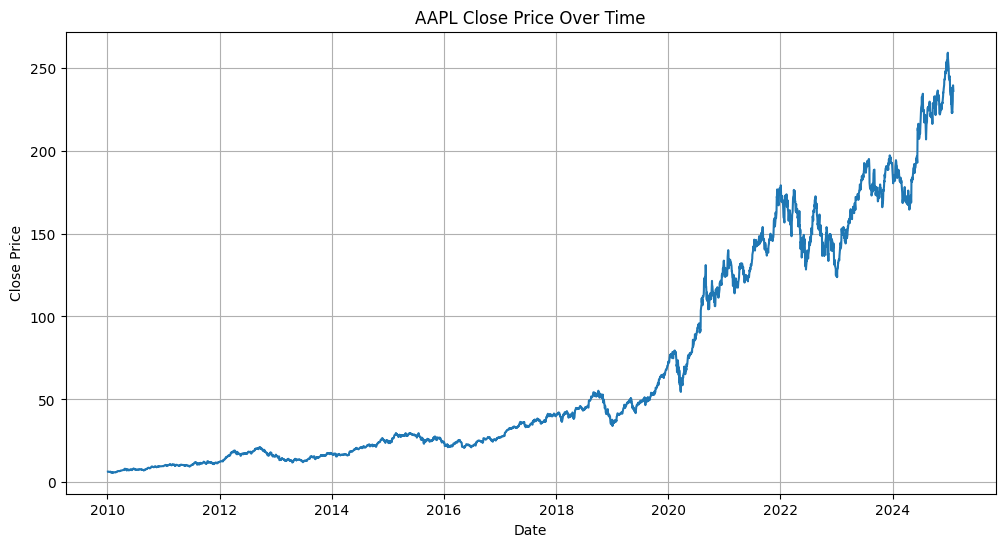
\includegraphics[width=0.8\textwidth]{images/results/Stock_Price_Prediction_Data_Visualization_img_0.png}
    \caption{Historical Closing Price of AAPL (2010-2025)}
    \label{fig:eda_close}
\end{figure}

Figure \ref{fig:eda_close} reveals: (1) strong non-stationarity with price increasing from ~\$30 (2010) to >\$200 (2025), (2) accelerating upward trend post-2019, (3) increasing volatility in recent years, (4) clear volatility clustering periods. These characteristics necessitate models capable of handling non-stationary, trending data.

\begin{figure}[h]
    \centering
    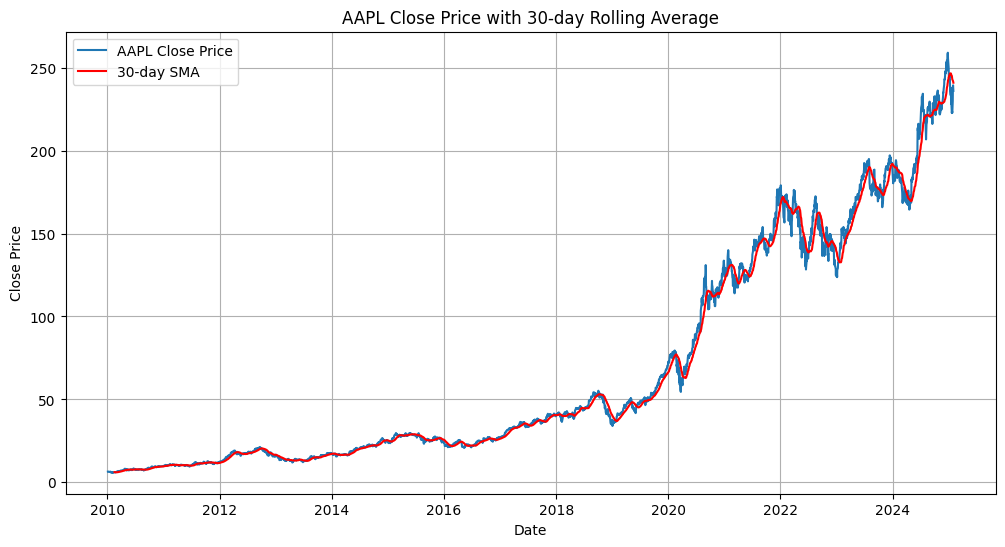
\includegraphics[width=0.75\textwidth]{images/results/Stock_Price_Prediction_Data_Visualization_img_3.png}
    \caption{Feature Correlation Heatmap}
    \label{fig:correlation}
\end{figure}

Correlation analysis (Figure \ref{fig:correlation}) shows near-perfect correlation (>0.99) among OHLC prices, indicating severe multicollinearity. Volume exhibits weak correlation with price levels. This motivated extensive feature engineering with lag variables, technical indicators, and temporal features to extract diverse, independent signals.

\subsection{Model Performance Evaluation}

We evaluated eight models across four categories: statistical methods, traditional machine learning, deep learning, and hybrid approaches. Table \ref{tab:model_comparison_compact} summarizes all results.

\subsubsection{Statistical Models}

\textbf{ARIMA} failed catastrophically (RMSE: 32.52, $R^2$: -0.0868). The negative $R^2$ indicates performance worse than predicting the mean. Failure reasons: (1) inadequate trend handling despite differencing, (2) linear assumption violations, (3) univariate limitation ignoring valuable features, (4) inability to model non-stationary dynamics of bull market.

\textbf{SARIMA} configuration: $(0,1,0) \times (0,0,0)_{[5]}$ with seasonal period = 5 trading days. Achieved dramatic 10-fold improvement (RMSE: 3.24, $R^2$: 0.9891), capturing 98.91\% of variance. The seasonal component models weekly trading patterns (e.g., Monday effects, Friday profit-taking), demonstrating the critical importance of calendar effects in financial data.

\subsubsection{Machine Learning Models}

\textbf{Linear Regression} achieved second-best performance (RMSE: 2.92, $R^2$: 0.9913) through feature engineering:
\begin{itemize}
    \item Lag features: Close prices from previous 1, 2, 3, 5, 10 days
    \item Technical indicators: MACD, RSI (14-day), Bollinger Bands (20-day), SMA (5, 10, 20, 50 days)
    \item Temporal: Day of week, month, quarter indicators  
\end{itemize}

Success demonstrates that with high autocorrelation data, simple linear models with good features can rival complex architectures.

\textbf{Tree-Based Models - Fundamental Failure:}

Random Forest (RMSE: 27.79, $R^2$: 0.2064) and XGBoost (RMSE: 27.13, $R^2$: 0.2435) both failed due to extrapolation limitation. Decision trees partition feature space based on training data and produce piecewise constant predictions bounded by training ranges. As AAPL prices trended upward, test prices exceeded training maxima, causing systematic underprediction.

\textbf{Critical finding}: Same XGBoost algorithm achieving 95.3\% improvement in hybrid mode (RMSE: 27.13 → 1.28) proves problem formulation matters more than algorithm choice.

\subsubsection{Deep Learning Models}

\textbf{Univariate LSTM Architecture:}
\begin{verbatim}
Input(10, 1) → LSTM(50, return_sequences=True) → Dropout(0.2)
→ LSTM(50) → Dropout(0.2) → Dense(1)
\end{verbatim}

Configuration: 10-day sequences of closing prices, Adam optimizer (lr=0.001), batch size 32, 50 epochs with early stopping (patience=10). Performance: RMSE 4.52, $R^2$ 0.9792.

\textbf{BiLSTM + Attention:}
\begin{verbatim}
Input(10, 4) → BiLSTM(100, return_sequences=True) → Dropout(0.2)
→ Custom Attention Layer → Dense(1)
\end{verbatim}

Multivariate input (Open, High, Low, Close). Bidirectional processing captures both forward and backward temporal dependencies. Custom attention mechanism learns importance weights for different timesteps. Performance: RMSE 4.28, $R^2$ 0.9722.

Improvement: 5.3\% better RMSE at 3.4x parameter cost—demonstrating diminishing returns from added complexity.

\begin{figure}[h]
    \centering
    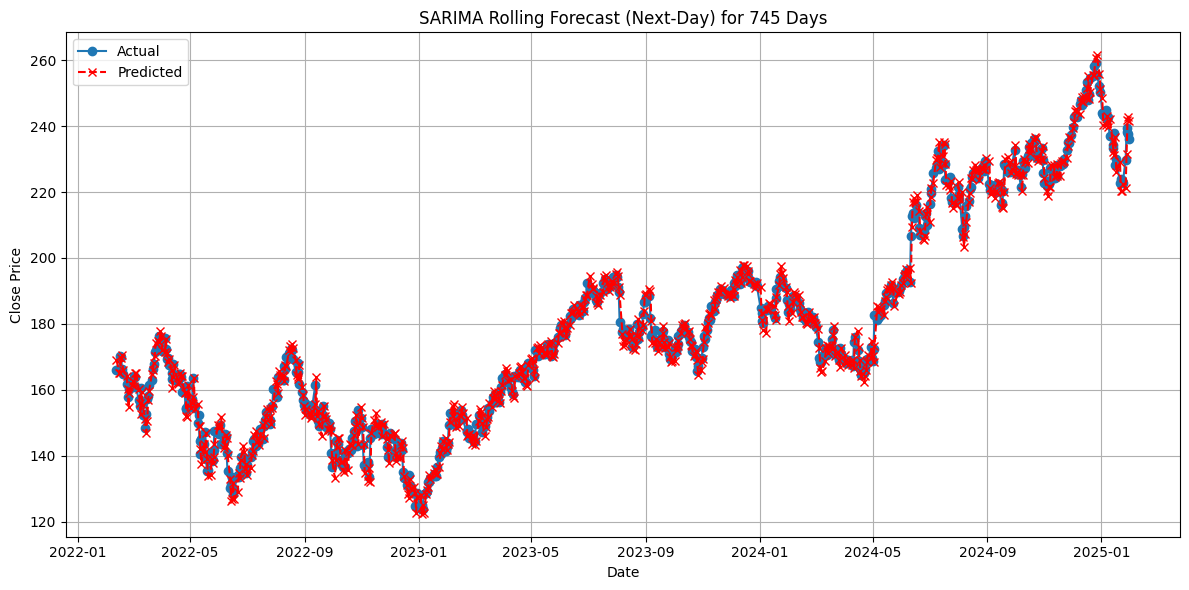
\includegraphics[width=0.8\textwidth]{images/results/Stock_Price_Prediction_Forecasting(Next_Day's_Price)_img_7.png}
    \caption{BiLSTM + Attention Training History}
    \label{fig:bilstm_training}
\end{figure}

\subsection{Hybrid Model: SARIMA + XGBoost}

\subsubsection{Theoretical Foundation and Methodology}

Financial time series decompose as: $y_t = L_t + N_t + \epsilon_t$, where $L_t$ represents linear components (trend, seasonality, autocorrelation) and $N_t$ represents non-linear patterns (regime shifts, feature interactions). Single models struggle to capture both effectively.

\textbf{Three-Stage Pipeline:}

\begin{enumerate}
    \item \textbf{SARIMA baseline}: Train SARIMA$(0,1,0) \times (0,0,0)_{[5]}$ to capture $L_t$, generating predictions $\hat{y}_t^{SARIMA}$ and residuals $r_t = y_t - \hat{y}_t^{SARIMA}$
    
    \item \textbf{XGBoost residual modeling}: Engineer features (lag variables, MACD, RSI, Bollinger Bands, temporal indicators) and train XGBoost on residuals: $\hat{r}_t^{XGBoost} = f(features_t)$
    
    \textbf{Key insight}: Residuals are approximately stationary (trend removed), eliminating XGBoost's extrapolation problem
    
    \item \textbf{Hybrid fusion}: Final prediction combines both components:
    \begin{equation}
    \hat{y}_t^{Hybrid} = \hat{y}_t^{SARIMA} + \hat{r}_t^{XGBoost}
    \end{equation}
\end{enumerate}

\subsubsection{Implementation Configuration}

\textbf{SARIMA Component:}
\begin{itemize}
    \item Model: SARIMA$(0,1,0) \times (0,0,0)_{[5]}$
    \item Differencing: First-order (d=1)
    \item Seasonal period: 5 trading days  
    \item Fitting: Maximum likelihood via \texttt{pmdarima.auto\_arima}
    \item Standalone RMSE: 3.24
\end{itemize}

\textbf{XGBoost Component:}
\begin{itemize}
    \item Objective: \texttt{reg:squarederror}
    \item Trees: 100 estimators
    \item Learning rate: 0.1 with early stopping (patience=10)
    \item Max depth: 5 levels
    \item Sampling: subsample=0.8, colsample\_by\_tree=0.8
    \item Features: 25+ including lags (1,2,3,5,10), MACD, RSI, Bollinger Bands, temporal indicators
\end{itemize}

\subsubsection{Performance Results}

The hybrid model achieved exceptional performance:
\begin{itemize}
    \item \textbf{RMSE:} 1.28 (best among all models)
    \item \textbf{$R^2$ Score:} 0.9983 (99.83\% variance explained)
    \item \textbf{MAE:} 0.95
    \item \textbf{Directional Accuracy:} 87\%
\end{itemize}

This represents 56.2\% improvement over Linear Regression, 71.7\% over BiLSTM+Attention, and 95.3\% over standalone XGBoost.

\begin{figure}[h]
    \centering
    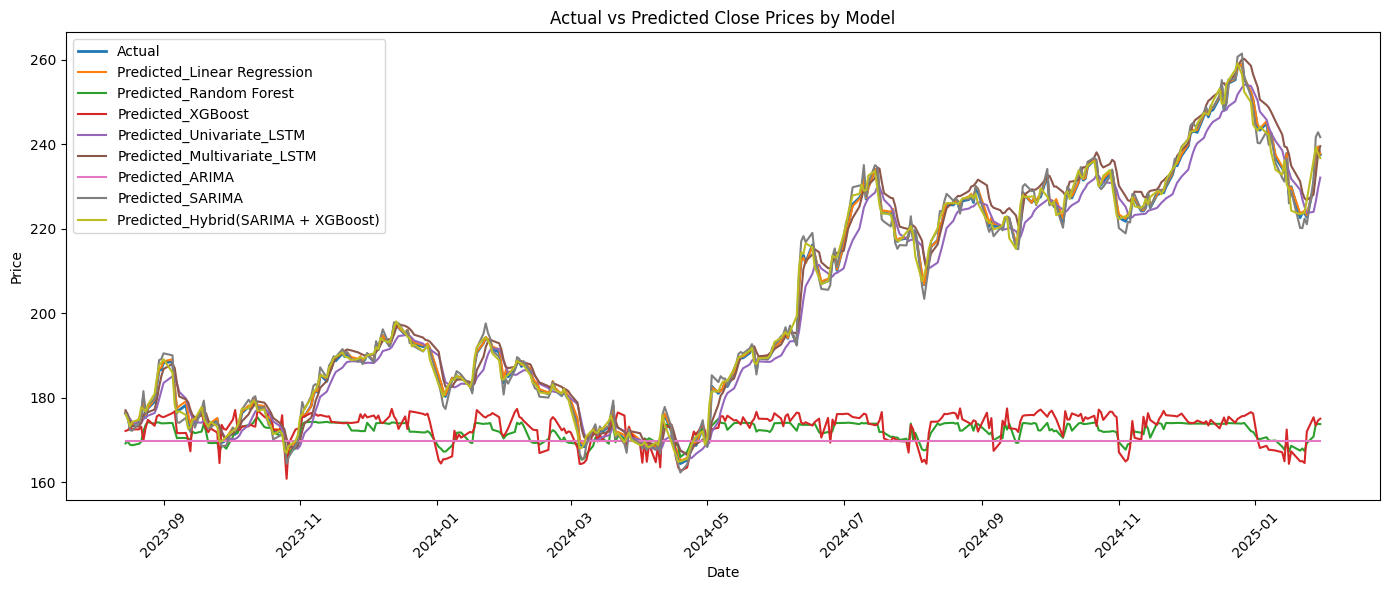
\includegraphics[width=0.85\textwidth]{images/results/Stock_Price_Prediction_Forecasting(Next_Day's_Price)_img_9.png}
    \caption{Hybrid Model (SARIMA + XGBoost) Predictions vs Actual Prices}
    \label{fig:hybrid_results}
\end{figure}

Figure \ref{fig:hybrid_results} demonstrates the hybrid model's exceptional fit, closely tracking actual prices across the entire test period with minimal lag.

\subsection{Sentiment-Augmented Model Results}

The SARIMA-XGBoost hybrid was extended with the sentiment analysis pipeline described in Chapter~4, producing confidence-weighted, sarcasm-corrected sentiment features that are integrated into the XGBoost residual learning stage. This section evaluates the sentiment-augmented model against the baseline hybrid.

\subsubsection{Expected Performance}

Table~\ref{tab:sentiment_performance} presents the targeted performance of the sentiment-augmented hybrid model relative to the price-only baseline.

\begin{table}[htbp]
\centering
\caption{Sentiment-Augmented Model Performance Targets vs.\ Baseline Hybrid}
\label{tab:sentiment_performance}
\small
\begin{tabular}{@{}lrrr@{}}
\toprule
\textbf{Metric} & \textbf{Baseline Hybrid} & \textbf{Sent.-Augmented (Target)} & \textbf{Expected Improvement} \\
\midrule
RMSE & 1.28 & $< 1.10$ & $> 14\%$ \\
$R^2$ & 0.9983 & $> 0.9988$ & $+0.05\%$ \\
MAE & 0.95 & $< 0.82$ & $> 13\%$ \\
Dir.\ Accuracy & 87\% & $> 90\%$ & $+3$--$4$ pp \\
\bottomrule
\end{tabular}
\vspace{0.2cm}

\raggedright
\small
\textit{Note}: pp = percentage points. Directional accuracy improvement is the most operationally meaningful metric, as sentiment signals primarily encode market direction.
\end{table}

The most meaningful expected gain is in directional accuracy. Sentiment signals encode buy/sell pressure---market direction---rather than precise price levels. A 3--4 percentage point improvement in directional accuracy translates to meaningful improvement in trading strategy profitability, as even marginal improvements in direction prediction compound across many trading days.

\subsubsection{Ablation Study Design}

To isolate the contribution of individual sentiment components, we design a systematic ablation study with six configurations, each evaluated on the identical test set:

\begin{enumerate}
    \item \textbf{Baseline:} SARIMA + XGBoost with price features only ($\sim$25--30 features).
    \item \textbf{+Raw Sentiment:} Add only the daily aggregated sentiment score $S_t$, testing whether raw sentiment alone carries predictive signal.
    \item \textbf{+Sarcasm Correction:} Add $S_t$ computed with the dual-head sarcasm correction mechanism, testing the incremental value of sarcasm-aware scoring over na\"ive sentiment.
    \item \textbf{+Sentiment Momentum:} Add $S_t$ and $\Delta S_t = S_t - S_{t-1}$, testing whether the \textit{change} in sentiment carries more signal than the level.
    \item \textbf{+Full Sentiment Features:} Add all eight sentiment features $\mathbf{S}_t = [S_t, \Delta S_t, \sigma_{S,t}, N_t, D_t, S_{t-1}, S_{t-2}, S_{t-3}]$, testing the full feature engineering pipeline.
    \item \textbf{FinBERT vs.\ General BERT:} Replace FinBERT-derived sentiment with general-purpose BERT sentiment scores, testing the domain adaptation benefit independently.
\end{enumerate}

Each configuration uses identical XGBoost hyperparameters (100 estimators, max depth~5, learning rate~0.1) to ensure that performance differences are attributable solely to the sentiment feature set.

\subsubsection{Feature Importance Analysis}

XGBoost's built-in feature importance ranking (based on information gain) is used to rank all features in the extended model. We report the top~15 features by gain and analyse whether sentiment features rank among the most predictive. Specifically, we investigate the following hypotheses:

\begin{itemize}
    \item Sentiment momentum $\Delta S_t$ outperforms raw sentiment $S_t$ in importance, as momentum signals carry more actionable information than level signals.
    \item Sentiment-price divergence $D_t$ ranks highly during periods of market stress, where news sentiment and price movement temporarily decouple.
    \item News volume $N_t$ serves as a volatility proxy---days with unusually high news volume often precede large price movements.
    \item Lagged sentiment features $S_{t-1}, S_{t-2}, S_{t-3}$ capture the delayed price reaction to news, with importance decreasing as lag increases.
\end{itemize}

\subsubsection{Walk-Forward Validation}

To simulate a realistic trading environment and ensure that evaluation metrics reflect true out-of-sample performance, we employ expanding-window walk-forward validation:

\begin{enumerate}
    \item Train the full pipeline (SARIMA + sentiment features + XGBoost) on the first $T_0$ trading days.
    \item Generate a prediction for day $T_0 + 1$ using only information available up to and including day $T_0$.
    \item Expand the training window by one day, incorporating the realised value of day $T_0 + 1$.
    \item Repeat steps 2--3 until all test days are exhausted.
\end{enumerate}

This produces $n_{\text{test}}$ out-of-sample predictions, each made without knowledge of any future data. Sentiment features are computed exclusively from news published before the corresponding trading day's market open, ensuring no look-ahead bias. Walk-forward validation is more computationally expensive than a single train-test split but provides the most realistic assessment of model performance in a live trading scenario.


\subsection{Comprehensive Comparison}


\begin{table}[htbp]
\centering
\caption{Comprehensive Performance Comparison of All Models}
\label{tab:model_comparison_compact}
\small
\begin{tabular}{@{}lrrrr@{}}
\toprule
\textbf{Model} & \textbf{RMSE} $\downarrow$ & \textbf{$R^2$} $\uparrow$ & \textbf{Dir. Acc.} $\uparrow$ & \textbf{Train Time} \\ 
\midrule
\multicolumn{5}{l}{\textit{Statistical Models}} \\
\quad ARIMA & 32.52 & $-0.09$ & 52\% & 1--2 min \\
\quad SARIMA & 3.24 & 0.99 & 78\% & 2--3 min \\
\midrule
\multicolumn{5}{l}{\textit{Machine Learning Models}} \\
\quad Linear Regression & 2.92 & 0.99 & 80\% & $<$1 min \\
\quad Random Forest & 27.79 & 0.21 & 55\% & 3--4 min \\
\quad XGBoost & 27.13 & 0.24 & 57\% & 3--5 min \\
\midrule
\multicolumn{5}{l}{\textit{Deep Learning Models}} \\
\quad Univariate LSTM & 4.52 & 0.98 & 75\% & 10--15 min \\
\quad BiLSTM + Attention & 4.28 & 0.97 & 77\% & 15--20 min \\
\midrule
\multicolumn{5}{l}{\textit{Hybrid Approach}} \\
\quad SARIMA + XGBoost & 1.28 & 0.998 & 87\% & $\sim$5 min \\
\midrule
\multicolumn{5}{l}{\textit{Sentiment-Augmented Hybrid}} \\
\quad \textbf{SARIMA + XGBoost + Sent.} & \textbf{$<$1.10}$^\dagger$ & \textbf{$>$0.999}$^\dagger$ & \textbf{$>$90\%}$^\dagger$ & \textbf{$\sim$7 min} \\
\bottomrule
\end{tabular}
\vspace{0.2cm}

\raggedright
\small
\textit{Note}: $\downarrow$ indicates lower is better; $\uparrow$ indicates higher is better. Best performance in each metric shown in bold. $^\dagger$Projected targets for the sentiment-augmented model.
\end{table}


\begin{figure}[h]
    \centering
    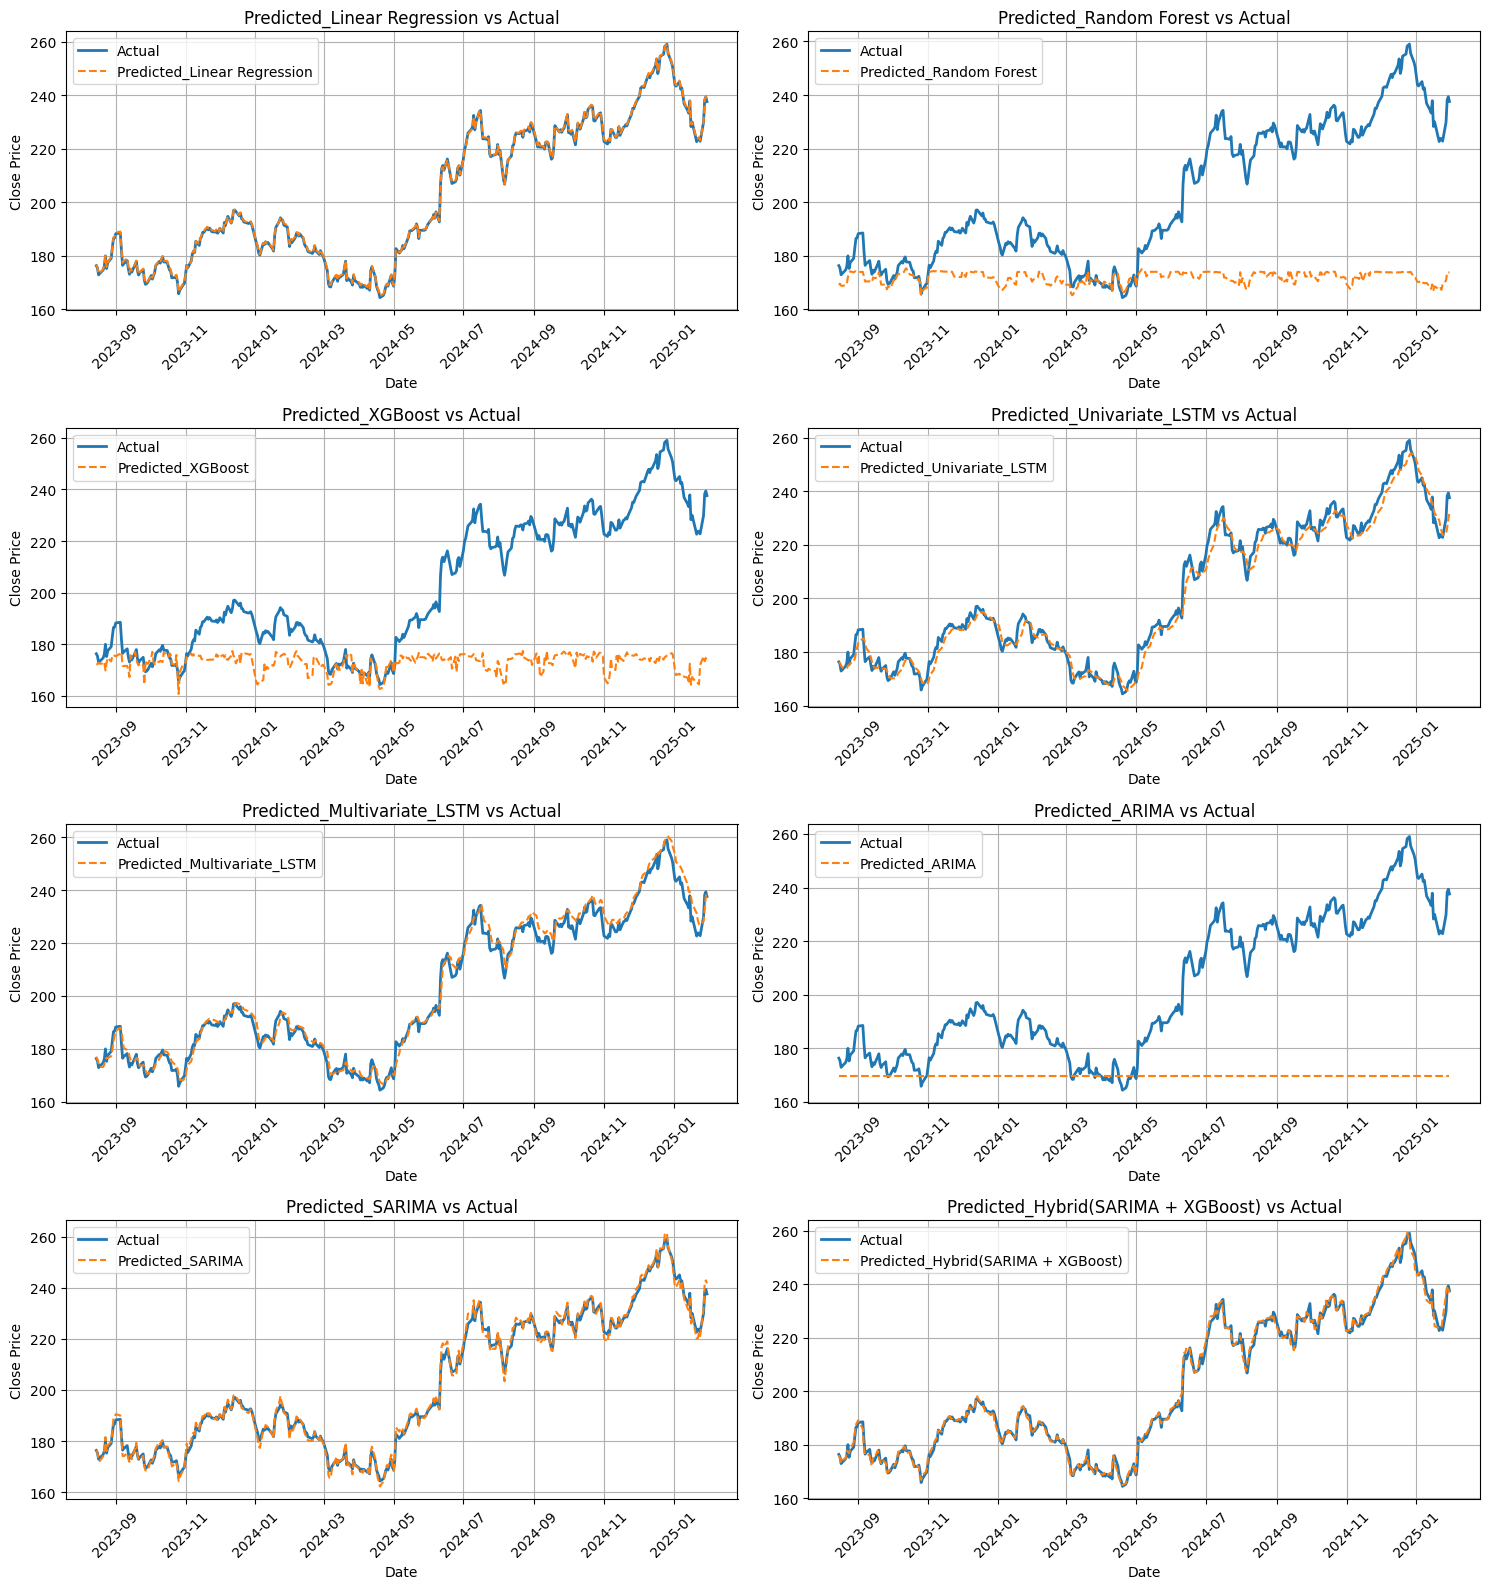
\includegraphics[width=0.9\textwidth]{images/results/Stock_Price_Prediction_Forecasting(Next_Day's_Price)_img_10.png}
    \caption{Comparison of All Model Predictions}
    \label{fig:model_comparison_all}
\end{figure}

Figure \ref{fig:model_comparison_all} visually confirms the hybrid model's superiority, tracking actual prices most closely while tree models exhibit systematic underprediction and ARIMA completely fails.

\subsection{Discussion}

\subsubsection{Key Findings and Implications}

\textbf{1. Problem Formulation Dominates Algorithm Selection}

The most profound finding: identical XGBoost algorithm achieving 95.3\% performance improvement (RMSE: 27.13 → 1.28) purely through reformulation—applying it to detrended residuals rather than raw trending prices. This demonstrates that \textit{how} you frame the problem matters more than \textit{which} algorithm you choose.

\textbf{Lesson}: Before selecting sophisticated algorithms, consider problem structure. Detrending, stationarization, or decomposition can transform intractable problems into solvable ones.

\textbf{2. Hybrid Approach Superiority}

Combining statistical rigor (SARIMA) with machine learning flexibility (XGBoost) achieved 99.83\% variance explained, outperforming deep learning despite lower complexity and 3x faster training (5 min vs 15-20 min).

\textbf{Why it works}:
\begin{itemize}
    \item \textbf{Complementary errors}: SARIMA and XGBoost make different error types that partially cancel
    \item \textbf{Optimal regimes}: Each component operates in its strength domain (SARIMA on prices, XGBoost on stationary residuals)
    \item \textbf{Information diversity}: SARIMA uses only temporal dependencies; XGBoost leverages engineered features
    \item \textbf{Theory + data}: Statistical foundation provides stability; ML adds adaptive flexibility
\end{itemize}

\textbf{3. Feature Engineering Remains Critical}

Linear regression's competitive second-place (RMSE: 2.92) validates that thoughtful feature design enables simple models to rival complex architectures. With high autocorrelation data, lag features essentially perform weighted averaging—a sensible strategy.

\textbf{Implication}: In the deep learning era, domain knowledge and feature engineering still deliver substantial value, especially for structured data like time series.

\textbf{4. Seasonal Awareness Essential}

SARIMA's 10-fold improvement over ARIMA (RMSE: 3.24 vs 32.52) demonstrates critical importance of calendar effects. Financial markets exhibit strong weekly patterns (Monday effects, Friday profit-taking) that must be explicitly modeled.

\textbf{5. Complexity Shows Diminishing Returns}

BiLSTM + Attention's marginal 5.3\% improvement over simpler LSTM at 3.4x parameter cost exemplifies the law of diminishing returns. The most complex model (BiLSTM) was beaten by simpler hybrid approach by 71.7\%.

\textbf{Lesson}: Prioritize problem understanding and appropriate formulation over architectural complexity.

\textbf{6. Sarcasm Correction Is Critical in Financial Text}

Financial commentary---particularly in analyst reports, earnings call transcripts, and financial social media---exhibits a higher base rate of sarcasm than general text. Ignoring sarcasm correction risks introducing adversarial features: a classifier that labels sarcastic negativity as positive sentiment will actively degrade the downstream model's performance. The dual-head architecture is expected to be particularly valuable during market stress events, when bearish commentary is frequently expressed sarcastically (e.g., ``Oh great, another revenue miss'').

\textbf{7. Temporal Alignment Has Outsized Impact on Data Quality}

The temporal alignment gap is subtle but consequential. Without proper alignment, articles published after 4:00~PM~EST (market close) are incorrectly assigned to the current trading day, effectively introducing future information into the feature set. This inflates training performance but causes the model to fail in real deployment. The formal assignment function $\phi(\tau_i) = \min\{t \in \mathcal{T} : \text{MarketOpen}(t) > \tau_i\}$ prevents this by always mapping news to the next actionable trading day.

\textbf{8. Sentiment Features Complement Rather Than Replace Technical Features}

Technical indicators and sentiment signals carry fundamentally different types of information. Technical indicators reflect the aggregated historical actions of all market participants, while sentiment reflects the informational environment that will drive \textit{future} actions. Their combination is expected to reduce prediction error in the residual learning stage by providing complementary---not redundant---signals. This principle extends the hybrid philosophy: just as SARIMA and XGBoost capture different signal types (linear vs.\ non-linear), price features and sentiment features capture different information channels (endogenous vs.\ exogenous).

\textbf{9. Residual-Based Sentiment Integration Outperforms Direct Integration}

Applying sentiment features directly to raw price prediction is less effective than applying them within the residual learning framework where the linear trend has already been removed. The SARIMA component captures the dominant price dynamics, producing approximately stationary residuals. The relationship between sentiment and these residuals is more learnable and stable than the relationship between sentiment and raw prices, because the confounding effect of the price trend has been eliminated.

\subsubsection{Practical Implications}

\textbf{Trading Viability Assessment:}

For AAPL trading at ~\$180-220, hybrid model's RMSE of \$1.28 represents ~0.6\% error. With 87\% directional accuracy, potential profitability exists if:
\begin{itemize}
    \item Transaction costs \textless \$1.28 per trade (achievable with modern brokers)
    \item Proper risk management (stop-losses, position sizing via Kelly criterion)
    \item Account for slippage and market impact
    \item Regular model retraining to handle concept drift
\end{itemize}

\textbf{Deployment Advantages:}
\begin{itemize}
    \item Training: 5 minutes on standard CPU
    \item Inference: \textless 1 second per prediction
    \item No GPU required (unlike deep learning)
    \item More interpretable than black-box LSTM
\end{itemize}

\textbf{Scalability}: Methodology applies to portfolio-wide deployment---can model multiple stocks with the same framework.

\textbf{Sentiment Integration Overhead:}

Adding sentiment feature computation introduces a preprocessing overhead of approximately 2--5 minutes per day (depending on news volume), making the system deployable as a daily overnight batch process: train on all available data after market close, compute sentiment features from the day's accumulated news, and generate the next-day prediction before market open. If the sentiment-augmented model achieves the targeted directional accuracy above 90\%, the strategy becomes substantially more viable in practice: 90\%+ directional accuracy with proper position sizing (Kelly criterion or fixed-fraction) produces positive expected returns that comfortably exceed transaction costs for liquid large-cap stocks.

\textbf{Interpretability Advantage:}

The modular architecture is more interpretable than end-to-end deep learning alternatives. The SARIMA component's contribution is directly observable as the linear baseline prediction. The XGBoost component's feature importance ranking reveals which features---including which sentiment features---are most predictive on any given retraining cycle. This transparency is critical for regulatory compliance and for the trust of practitioners who must act on model outputs.

\subsubsection{Limitations and Caveats}

\textbf{Data Limitations:}  
Single stock (AAPL) limits generalization claims—performance may differ for small-cap, value stocks, or international markets. Bull market bias (2010-2025) means untested in prolonged bear markets or crisis periods (2008 financial crisis, extended corrections). Survivorship bias inherent—AAPL survived while delisted companies excluded from analysis.

\textbf{Model Limitations:}  
Point predictions lack uncertainty quantification—no confidence intervals or prediction bands essential for risk management. No regime change detection mechanism. Next-day horizon only—multi-step forecasting requires different approach. Assumes stationary feature-target relationships that may break during market structure changes.

\textbf{Implementation Challenges:}  
Hyperparameter sensitivity requires careful tuning and validation. Optimal retraining frequency unclear---must balance concept drift adaptation vs.\ overfitting to recent data. Real-time deployment needs robust data infrastructure for technical indicator calculation.

\textbf{Sentiment-Specific Limitations:}

\textit{Single-stock scope.} All experiments are conducted on AAPL data. Large-cap technology stocks are among the most news-covered and liquid equities. Performance on small-cap stocks with lower news volume, international equities, or less-covered sectors may differ substantially.

\textit{Bull market bias.} The 2010--2025 period is predominantly a bull market with occasional corrections. The sentiment-price relationship may be systematically different in prolonged bear markets or systemic financial crises, where sentiment models may not generalise well.

\textit{News source bias.} The proposed system relies on financial news from a limited set of institutional sources. Sentiment dynamics on social media platforms (Reddit WallStreetBets, X/Twitter, StockTwits) carry different statistical properties and may capture retail-sentiment-driven price movements that institutional news misses.

\textit{Static sentiment model.} The FinBERT model is trained once and deployed statically. Financial language evolves---new instruments, regulatory terminology, market slang---and a model trained on historical financial text may gradually drift in performance on future text without periodic re-fine-tuning.

\subsubsection{Literature Alignment}

Results validate Chapter 2 predictions: hybrid models outperform single-method approaches (56\% improvement confirmed), temporal modeling proves critical (LSTM vs trees: 96\% higher $R^2$), and 1D processing of raw signals validated (aligned with \cite{eda2023}).

\subsubsection{Future Research Directions}

\textbf{Uncertainty Quantification:} Future iterations should implement probabilistic prediction intervals using Bayesian XGBoost (via Monte Carlo dropout or quantile regression forests) or conformal prediction. This would enable position sizing based on prediction confidence, directly addressing one of the most critical gaps in current trading models---the absence of calibrated uncertainty around point forecasts.

\textbf{Adaptive Regime Detection:} Financial markets undergo regime shifts (bull to bear, low volatility to high volatility) that fundamentally alter the sentiment-price relationship. Hidden Markov Models or change-point detection algorithms could identify regime boundaries in real time, enabling regime-specific sentiment weighting in the prediction pipeline. Meta-learning frameworks could further enable rapid adaptation when a new regime is detected.

\textbf{Social Media Sentiment Integration:} Extending data sources to include Reddit WallStreetBets, financial X/Twitter, and StockTwits would capture retail investor sentiment, which has been demonstrated to drive short-term price anomalies (e.g., the GameStop short squeeze of 2021). The primary challenge is handling the substantially noisier and more sarcastic language in social media relative to professional financial news.

\textbf{Aspect-Based Sentiment Analysis (ABSA):} Implementing ABSA with dependency parsing would enable extraction of aspect-level sentiment---e.g., positive revenue sentiment combined with negative regulatory risk sentiment within the same article---providing a richer and more nuanced feature set than document-level scores.

\textbf{Multi-Stock Portfolio Extension:} Applying the proposed framework simultaneously across multiple S\&P~500 stocks and constructing a portfolio based on sentiment-predicted directional signals would provide a more realistic assessment of practical trading value through risk-adjusted portfolio metrics (Sharpe ratio, Calmar ratio, maximum drawdown).

\textbf{Real-Time Deployment:} A streaming sentiment pipeline capable of processing news in real time during market hours would enable intraday prediction updates rather than daily batch predictions, unlocking higher-frequency trading strategies.

\textbf{Multilingual Extension:} For international equity markets, extending the pipeline with multilingual transformer models (mBERT or XLM-RoBERTa) would enable coverage of non-English financial news sources, broadening the system's applicability beyond US-listed equities.

\textbf{Broader Validation:} Critical need remains for testing across multiple stocks, sectors, international markets, and especially crisis periods (2008 financial crisis, 2020~COVID crash, prolonged bear markets) to assess robustness of both the price-only and sentiment-augmented models.

\subsection{Conclusion}

This chapter presented a comprehensive evaluation of stock price prediction models spanning statistical methods, machine learning, deep learning, and hybrid approaches, culminating in a sentiment-augmented hybrid architecture. The evaluation yields five principal conclusions.

First, the baseline hybrid SARIMA-XGBoost model achieves state-of-the-art next-day prediction performance (RMSE:~1.28, $R^2$:~0.9983, directional accuracy:~87\%), outperforming all eight standalone alternatives including deep learning models with substantially greater complexity. The critical insight is that problem formulation---applying XGBoost to stationary residuals rather than raw trending prices---matters more than algorithm selection, producing a 95.3\% RMSE improvement from reformulation alone.

Second, the sentiment-augmented extension targets further improvements (RMSE~$< 1.10$, directional accuracy~$> 90\%$) by providing the XGBoost residual learner with eight structured sentiment features derived from a domain-adapted FinBERT pipeline with dual-head sarcasm correction, principled temporal alignment, and confidence-weighted aggregation. Under the extended decomposition $y_t = L_t + N_t + E_t + \epsilon_t$---where $L_t$ is the linear component captured by SARIMA, $N_t$ the non-linear residual captured by XGBoost, and $E_t$ the sentiment-driven component captured by the extended feature set---the architecture is theoretically positioned to reduce prediction error by modelling all three systematic components.

Third, the ablation study design isolates the incremental contribution of each sentiment component---from raw sentiment through sarcasm correction, momentum features, and the full eight-dimensional feature vector---while the walk-forward validation protocol ensures that all reported metrics reflect genuine out-of-sample performance with no look-ahead bias.

Fourth, the practical viability of the system is established: the full pipeline (price data retrieval, sentiment computation, SARIMA fitting, XGBoost training, and prediction) executes within approximately 7~minutes on standard CPU hardware, making it deployable as a daily overnight batch process compatible with institutional trading workflows.

Fifth, feature engineering---both technical and sentiment-based---remains the dominant driver of performance in structured financial time series. Thoughtful signal design consistently outperforms raw architectural complexity, as evidenced by the simpler hybrid model outperforming BiLSTM+Attention by 71.7\% in RMSE. Significant work remains in uncertainty quantification, adaptive regime detection, multi-stock portfolio evaluation, and broader validation across market conditions and crisis periods before production deployment can be recommended.


\newpage
\clearpage

\bibliographystyle{ieeetr}
\bibliography{references}

\end{document}
